%To process your document use the following commands at the linux command line:
%                  latex filename
%to produce a DVI file called filename.dvi which you can view using the command
%                  xdvi filename1 &
%To print the dvi file, type
%                  dvips -Pyourprintername filename
%If you want to convert the dvi file to PDF format, type
%                  dvips -o filename.ps filename
%which will create a PS file called filename.ps. And then type
%                  ps2pdf filename.ps
%which will create a PDF file called filename.pdf, which you can view with the acrobat reader. 
%You can also use
%                  pdflatex filename
% to convert your latex file filename.tex directly into PDF format without producing the DVI and PS files, but that doesn't work if you have graphs.
%If you're using a version of latex for Windows you can usually run these commands from the pulldown menu of your editor. You need to install a DVI viewer to view the DVI file and  Ghostview to view the PS files. These can be found in various places online. You may be able to process the latex file and turn it into a PDF file directly.


\documentclass[12pt]{article}
\usepackage{graphicx}  
\usepackage{graphics}
%\setcounter{secnumdepth}{1}
\usepackage{amssymb}
\usepackage{amsmath}
\usepackage{siunitx} 
\usepackage [english]{babel}
\usepackage [autostyle, english = american]{csquotes}
\usepackage{amsthm}
\usepackage[strict]{changepage}
\usepackage{relsize}
\usepackage{nccmath}
\usepackage{mathtools}
\usepackage{multicol}
\usepackage{epstopdf}




\newtheorem{theorem}{Theorem}[section]
\newtheorem{definition}{Definition}[section]
\newtheorem{corollary}{Corollary}[theorem]
\newtheorem{lemma}[theorem]{Lemma}
\theoremstyle{definition}
\newtheorem*{remark}{Remark}
\numberwithin{equation}{section}

%Adjust these numbers to change the size of your margins
\setlength{\textheight}{210mm}
\setlength{\topmargin}{-5mm}
%\setlength{\footskip}{-5mm}
\setlength{\textwidth}{145mm}
\setlength{\oddsidemargin}{12mm}

\epstopdfsetup{outdir=./figures}  %Required to change filepath for .eps graphics because exectuing typesetting uses the {epstopdf} package to convert .eps graphics to .pdf format.
\graphicspath{{figures/}}	%Ensures that .eps graphics used for figures is found at the appropriate path.

\renewcommand{\baselinestretch}{1.5} %%%% Comment this out to produce a single-spaced document. For double-spacing use 1.5 or 2.0.

\begin{document}

%\begin{titlepage}

%\large

%\begin{center}
%{\LARGE Linear Dispersive Waves in Optical Fibers}

%\vspace{20mm}

%{\Large By: Tommy Zieba}

%\vspace{20mm}
%{\Large Carleton University - School of Mathematics and Statistics}
%\vspace{120mm}
%{\large Honours Project Report}

%{\large April 25, 2018}
%\end{center}



%\end{titlepage}



\pagebreak
\pagenumbering{roman}

%\renewcommand{\baselinestretch}{1.5} 
\tableofcontents
\addtocontents{toc}{\contentsline {section}{\numberline {}Abstract}{1}}
%%\addtocontents{toc}{\contentsline {section}{\numberline {}Acknowledgements}{iv}}
%%\addtocontents{toc}{\contentsline {section}{\numberline {}List of figures}{vii}}
%%\addtocontents{toc}{\contentsline {section}{\numberline {}List of symbols}{xii}}

%%\listoffigures
\newpage


\begin{center}

{\Large \bf Abstract}
\end{center}
Optical fibers are used primarily for transmitting information. The theory of optical fibers provides methods for transferring more information over a longer distance than traditional data transmission methods. This is due to the dispersive properties of light propagating through an optical fiber. In this report, the fundamental theory of linear dispersion over short distances in optical fibers is established. The differential equations and boundary conditions permitting light propagation in an optical fiber are derived. The theory of linear dispersive waves and group velocity are introduced. The method of characteristics is used to determine the characteristic equations which possible solutions must satisfy. We discuss the dispersion and group velocity behaviour of possible solutions satisfying the wave equation and characteristic equations. The theory of linear dispersion in optical fibers over short distances is useful for practical applications involving transmission of information. The theory of linear dispersive waves in optical fibers also leads to the study of non-linear effects in optical fibers.
\pagebreak
\pagenumbering{arabic}
\section{Introduction}
This report describes the propagation of light waves in an optical fiber. First, the topics that are discussed in this report are described and then an overview is given of the sections where these topics are described. The part of the optical fiber where wave propagation occurs is within its cylindrical glass core. Waves describing oscillations in space are represented by oscillatory functions of both space and time. In general, an oscillatory function represents a waveform that has a wavenumber that depends on position and a frequency that depends on time. An oscillatory function also has a phase which propagates with a phase velocity determined by the frequency and wavenumber.

Light propagation occurs in the optical fiber by the nature of the electric and magnetic fields, which determine how the positions of electrons may change with respect to changes time. Maxwell's equations govern the electric and magnetic fields in any material based on specifically and experimentally derived electric and magnetic field properties in the material. When light propagates through the fiber, the electric and magnetic fields describing the light behaves according to a wave equation, called Maxwell's wave equation, which has oscillatory solutions. 

Maxwell's wave equation is a second order partial differential equation (PDE) with respect to three dimensional position and time. In general, Maxwell's wave equation is a nonlinear PDE. The intensity of light propagating through the core corresponds to the varying amplitudes of the oscillatory solution to Maxwell's wave equation. Maxwell's wave equation takes the form of a linear PDE for sufficiently small intensities of light or for sufficiently small variations in the electric field distribution. These assumptions are necessary for finding possible linear dispersive solutions to Maxwell's wave equation using the method of characteristics.

A dispersive solution to a PDE is called hyperbolic at points where solutions exist and are uniquely determined by families of paths in the solution space. In general, hyperbolic PDEs are analyzed using the method of characteristics.

The second order wave equation is defined as a hyperbolic PDE. This is used to define Maxwell's wave equation as a second order wave equation with $4$ independent variables. The method of characteristics may be applied in general to find solutions to the $1$-dimensional wave equation to interpret the possible solutions to Maxwell's wave equation, which takes the form of a second order wave equation. Solutions to Maxwell's wave equation may take the form of a dispersive plane wave.

The definition of a dispersive equation and dispersive solutions are derived for general linear PDEs. When a differential equation has dispersive solutions, the solutions have oscillatory behaviour. We require a more general notion of phase, since it is changing as the solution oscillates. The relationship between wavenumber and frequency is generalized further by deriving the group velocity. Dispersion only occurs if the phase velocity is not the same as the group velocity. In other words, the average and local changes in phase are not the same.

Solutions to Maxwell's wave equation are derived by choosing boundary conditions that necessarily and sufficiently confine rays of light in the core. The characteristic equations corresponding to the paths of light rays in the solution of Maxwell's wave equation are derived from parametrizing light with linear rays. These characteristic equations represent differing modalities of light ray distribution within the core. The full dispersive solution for Maxwell's wave equation is a superposition of these modes. The example of a single type of light ray is presented as one of the possible modes satisfying the characteristic equation in section. 

Now, an overview of the topics mentioned above is given. The physical properties of an optical fiber and the properties of light within its glass core are described in section \ref{properties.sec}. The electric and magnetic fields and Maxwell's equations which describe them are defined in section \ref{maxwellsequations}. Before being able to define dispersion, the second order wave equation is defined as a hyperbolic PDE in section \ref{wave.sec}, where hyperbolic PDEs are discussed as well. This is required for existence of solutions to Maxwell's wave equation.

The method of characteristics is derived in appendix \ref{character.sec} and used in subsection 4.4 for the example of a 1-dimensional wave. Doing so leads to the definition of a plane wave in section \ref{wave.sec}, which is required in section \ref{guides.sec} for finding solutions that occur in this form. Before combining ideas from sections 1 to 4 to find solutions, dispersion, phase velocity and group velocity are defined in section 5.

Dispersion occurs only if the phase velocity is not the same as the group velocity. The dispersion is observed by finding solutions to Maxwell's wave equation in section \ref{guides.sec}
satisfying the linearization assumption, meaning that light is parametrized by rays. This only occurs for short distances in the optical fiber, since non-linear effects may emerge over a longer distance as it is inherent of the material properties. The approximation of the relative electric permittivity in subsection 3.2 allows for the linearization assumption.
\section{Properties of Optical Fibers}\label{properties.sec}
\subsection{Physical Properties}
These subsections follow \cite{Belanger}, \cite{Okamoto}, \cite{Reitz} and \cite{Partha}. There are several physical properties that an optical fiber possesses which must be considered. The isotropic, birefringent and homogeneous properties of the core are defined in this subsection. The main objective of this section is to define the specific properties of an optical fiber such that attenuation may be controlled by conditions at the core-cladding boundary. Attenuation is defined in subsection \ref{attenuation.sec}.

First, the microscopic and molecular structure of the glass core is characterized. An isotropic material is a material in which the physical properties do not depend on orientation, i.e. uniform structure. Glass is isotropic because the silica ($SiO_2$) molecules are arranged uniformly in a lattice that can be oriented symmetrically in any direction. It is possible, however, to manufacture optical fibers that include other compounds inducing a non-isotropic state in the glass.

Assume that there are no imperfections in the symmetry and no birefringence. Birefringence describes the affects of warping the cylindrical structure and is assumed to be neglected.

A homogeneous material has physical properties which do not depend on position. This report analyzes dispersion in a homogeneous optical fiber. It is possible, however, to manufacture optical fibers with physical properties that vary radially. The core of the optical fiber is covered by a material referred to as the cladding. The physical characteristics of the cladding are selected such that the attenuation in core may be controlled.

Refer to figure \ref{figure1} for an illustration of the optical fiber structure being considered. Note that the coating has no affect on the light propagation in the core and does not contribute to the boundary conditions at the core-cladding interface which we consider.
\begin{figure}[h!]
	\centerline{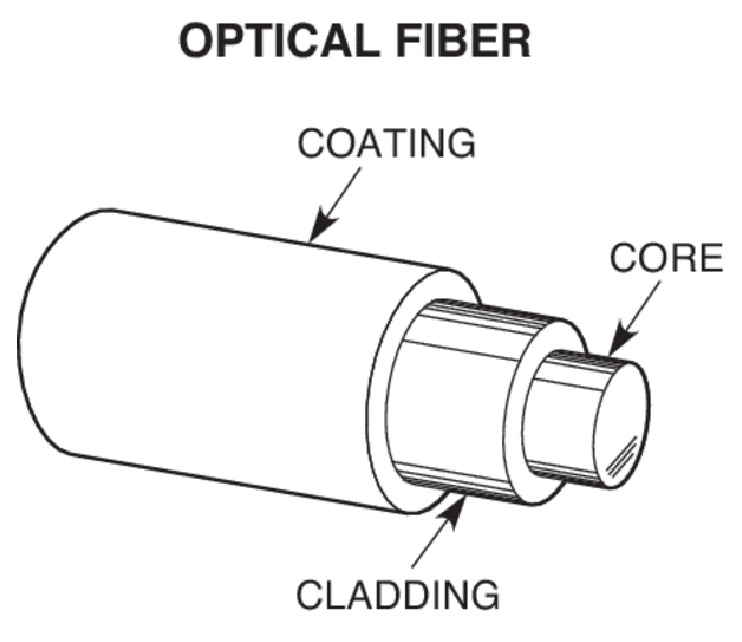
\includegraphics[height = 50mm, width=60mm, angle=0]{optical_fiber.eps}}
\caption{Optical fiber, \cite{fig_1}.}
\label{figure1}
\end{figure}

\subsection{Attenuation}\label{attenuation.sec}
The losses in an optical fiber refer to the forms in which loss of electric charge occurs when light propagates through the core. Generally, the attenuation in an optical fiber is derived from a reduction in the flux of the electric and magnetic field in a medium occurring. The electric and magnetic fields are defined in section \ref{maxwellsequations}. Molecules in the core reorient charges such that electromagnetic waves may propagate through it. In general, a loss of power occurs as electromagnetic waves propagate in the core and the wave becomes dissipated. A lossless medium is defined as one that does not suffer \textit{any} attenuation.

When light passes through any medium, the light is either reflected or absorbed according to the photoelectric effect. Otherwise, the light is reflected or refracted at the boundaries of the material according to Snell's law. The photoelectric effect and Snell's law accounts for all possible forms of attenuation in optical fibers.

The photoelectric effect is defined by the emission of electrons from a material when light is shined on it. This occurs in the valence orbital of atoms, which is not discussed further. Glass is a neutral material. This means valence orbitals of every atom are full as a consequence of $SiO_2$ molecules being bonded together in a lattice with shared valence electrons. Therefore, no electrons are reflected or absorbed due to the photoelectric effect. Moreover, the only form of attenuation occurring is refraction at the core-cladding boundary.
\subsection{Snell's Law and Total Internal Reflection}
Snell's law is the law governing refraction of light rays between materials, each having an associated index of refraction. Refraction refers to the path a ray of light takes when passing through a boundary between differing media. Before stating Snell's law, the definitions for a light ray and refractive index are required. Snell's law is used in this section to deduce the condition for total internal reflection. Total internal reflection refers to the phenomena of a light ray reflecting back into the incident media without refracting. Refer to figure \ref{figure3}. 

A light ray is defined by Descarte's law, which states that light travels along the path of least time. It may be proved, using variational calculus, that such a path is a straight line with respect to small variations on the proposed path \cite{Sagan}. A very crucial part of this proof is that it assumes a difference in time to occur if and only if there is at least one propagation direction. We do not show this proof; however, we assume such small variations and apply this as a necessary assumption in section \ref{guides.sec}. Snell's law follows from the variational proof and the fact that an extremum for the optical path is an extremum for the time taken as well.

The assumption of small variations in the light path corresponds to the linear approximation of permittivity, (defined in section \ref{maxwellsequations}), and implies that the refractive index in the glass core is constant. A materials refractive index is defined as the ratio of the speed of light in vacuum with the speed of light in the medium \textit{for small variations in the light path}. The speed of light in vacuum is given by $$c=\sqrt{\frac{1}{\varepsilon_0\mu_0}},$$ where the constants of permittivity, $\varepsilon_0$, and permeability, $\mu_0$, are defined in section \ref{maxwellsequations}. Refer to figure \ref{figure2} for the definition of Snell's Law. It states that
$$\frac{\sin{\theta_2}}{\sin{\theta_1}}=\frac{v_2}{v_1}=\frac{n_1}{n_0},$$
where $v_1$, $v_2$ is the phase velocity of light and $n_1$, $n_0$ is the refractive index in the media, respectively.
\begin{figure}[h!]
\centerline{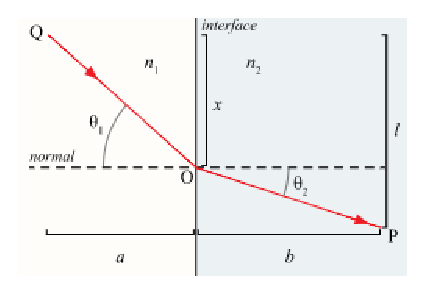
\includegraphics[height = 40mm, width=70mm, angle=0]{snellslaw2.eps}}
\caption{Snell's law, \cite{fig_2}.}
\label{figure2}
\end{figure}

From Snell's law, we may analyze the boundary conditions associated with solutions to the wave equation governing light propagation in the core. Light rays bend either away or toward the normal, relative to the incident ray direction, depending on which media has a higher refractive index. When rays move from higher to lower refractive index regions then light rays bend away from the normal. This is illustrated by figure \ref{figure3} for arbitrary refractive indices $n_1$ and $n_0$.
\begin{figure}[h!]
\centerline{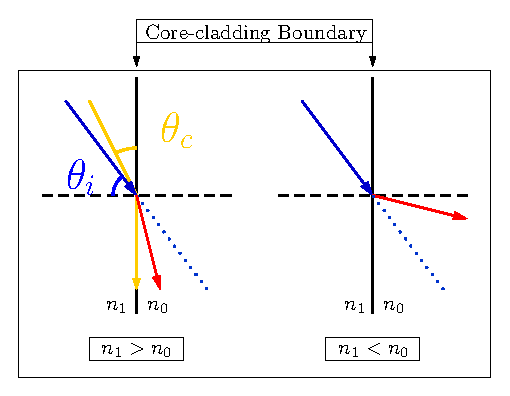
\includegraphics[height = 60mm, width=85mm, angle=0]{snell.eps}}
\caption{Refraction for relative differences in refractive index.}
\label{figure3}
\end{figure}

In order for rays with incident angles $0<\theta<\pi\slash 2$ to be reflected back into the core, the cladding must have a refractive index that is lower than the refractive index for glass. Let $n_1$ and $n_0$ be the refractive index for the core and cladding, respectively. We choose a material for the cladding such that $n_1>n_0$. Since the light rays bend away from the normal, there exists some angle where light begins to be reflected back into the incident media. This is called the critical angle. It is possible to use Snell's law to relate the critical angle, $\theta_c$, to the refractive indices by
\begin{equation}
\sin{\theta_c}=\frac{n_0}{n_1}.
\label{critical.eqn}
\end{equation}

Therefore, any angle larger than the the critical angle, given by (\ref{critical.eqn}), results in a refracted light ray. Now we check the maximum acceptance angle for totally reflected rays at the end face of the optical fiber based on the critical angle. Refer to figure \ref{figure4}.

\begin{figure}[h!]
\centerline{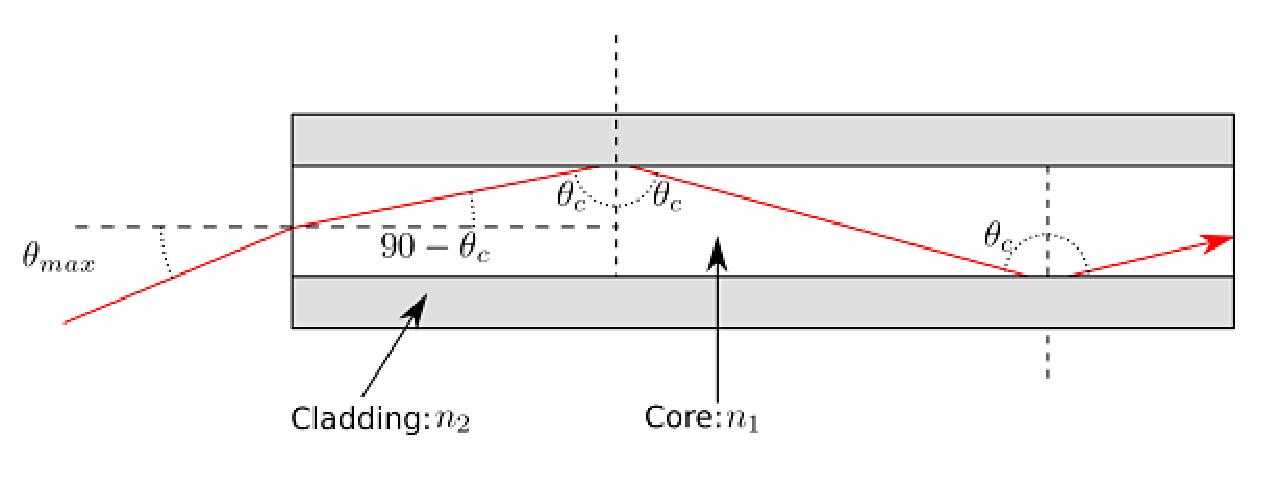
\includegraphics[height = 48mm, width=148mm, angle=0]{totalinternal.eps}}
\caption{Maximum acceptance angle, \cite{fig_4}.}
\label{figure4}
\end{figure}
Observe that the incident angle for rays within the core coming from the end right end face have an angle $\pi\slash 2-\theta_c$. Applying the critical angle condition from equation (\ref{critical.eqn}) with some trigonometric identities for angles $0<\theta_{max}<\pi\slash 2$ gives
$$\theta_{max}\leq\sin^{-1}{\sqrt{n_1^2+n_0^2}}.$$
Due to the cylindrical symmetry, this is the acceptance angle for which light rays are totally reflected in the core. Any light rays entering outside of the cone determined by the acceptance angle are refracted upon the first encounter with the core-cladding boundary and have no affect on the wave propagation in the core.
\subsection{Goss Hanchen Shift}
The only remaining physical phenomenon in optical fibers that needs to be accounted for as a boundary condition is a lateral shift called the Goss-Hanchen shift. It is observed experimentally and can be deduced mathematically by the derivations in \cite{Belanger} and \cite{Okamoto}. Light rays suffer a lateral shift upon reflection at the boundary. This lateral shift is due to a phase shift of the light ray whenever it is reflected at least twice. The following summarizes the arguments in \cite{Okamoto} and states the phase-matching condition at the core-cladding boundary.

The phase matching condition refers to the phase of a light ray propagating along the length of the core with an arbitrary planar phase surface. A phase surface is discussed in section \ref{dispersion.sec}. A ray of light is necessarily governed by Maxwell's equation described in section \ref{maxwellsequations}.

Due to the assumption of small variations in the path of light, (which defines a ray of light), different points on the same planar phase surfaces may have to traverse longer geometrical distance in the same time. These distances are the supposed paths of light rays. The light rays cannot bend while propagating in the core alone, but when reflected from the boundary, the magnetic field at every point of the ray rotates an angle $\pi\slash 2$.

The resulting light ray suffers a complex phase shift according to the angle of incidence. The phase difference may be interpreted by considering the reflected magnetic field components of the light ray in superposition with the reflected electrical field components. The electric and magnetic field are defined in section \ref{maxwellsequations}. The phase shift of the magnetic field is illustrated in figure \ref{figure5} and \ref{figure6}.
\begin{figure}[h!]
\centerline{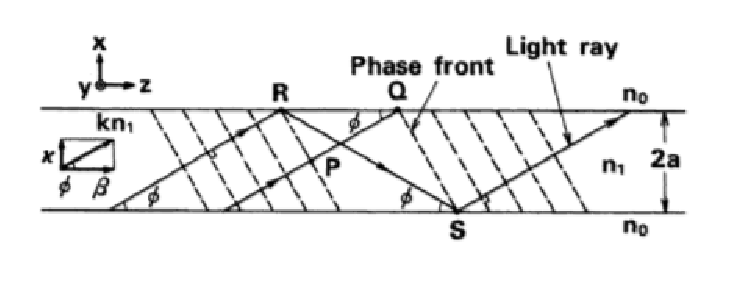
\includegraphics[height = 35mm, width=100mm, angle=0]{okamoto_fig1_2.eps}}
\caption{Light ray propagation for planar phase surfaces, \cite{Okamoto}, page 2.}
\label{figure5}
\end{figure}
\begin{figure}[h!]
\centerline{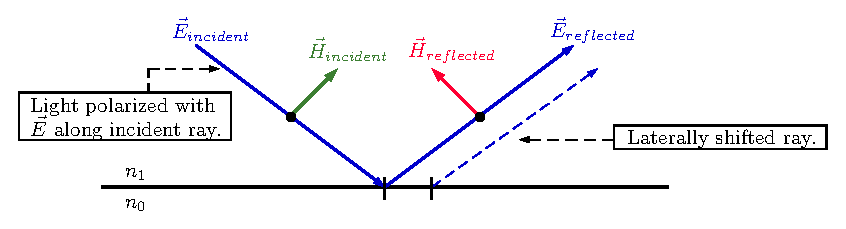
\includegraphics[height = 40mm, width=140mm, angle=0]{lightRayPropagation.eps}}
\caption{Demonstrating the need for phase matching condition.}
\label{figure6}
\end{figure}
We now state the phase matching condition according to figure \ref{figure5} and figure \ref{figure6}. Let $kn_1$ be the wavenumber for the phase of incident ray having angle $\phi$ and let $\beta$ be the component of the wavenumber in the $z$ direction as in firgure 5. The phase matching condition is given as 
\begin{equation}
\tan{\left(kn_1a\sin{\phi}-\frac{m\pi}{2}\right)}=\sqrt{\frac{2\left(\frac{n_1^2-n_0^2}{2n_1^2}\right)}{\sin^2{\phi}}-1},
\label{phasematch.eqn}
\end{equation}
where phase fronts are perpendicular to the path of a light ray propagating with wavelength and wavenumber $\lambda\slash n_1$ and $kn_1=2\pi n_1\slash\lambda$, respectively. Note that $\lambda$ denotes the wavelength of light in vacuum. It is important to point out that a light ray propagates on a planar phase front along the $z$ direction with respect to the equation
$$\beta=kn_1\cos{\phi}.$$

The phase matching condition implies that light ray propagation is discrete and is determined by the radius, refractive indices, and wavelength $\lambda$. In order for light rays to be confined within the core, the phase matching condition must be satisfied.
\section{Introducing Maxwell's Equations}
\label{maxwellsequations}
The subsections here mainly follow \cite{Reitz} with some interpretation from \cite{Flei}. Maxwell's equations are a set of four differential equations. The objective of section \ref{maxwellsequations} is to derive Maxwell's equations from various experimental and mathematical results. The four equations will be derived and stated individually throughout the following subsections. The equations describe the local behaviour of time dependent electric and magnetic fields in 3-dimensional space.

Let $S$ be a surface which encloses an arbitrary volume in 3-dimensional space that includes the origin. Let the set of points contained in the volume and on $S$ be denoted by $V$. The electric and magnetic fields are vector fields associated with the points in $V$. The electric field is defined in section \ref{gausseleclaw} and the magnetic field is defined in section \ref{mag_induction.sec}.

Maxwell's equations describe these two vector fields and provides relations involving the electric and magnetic fields with respect to position in $V$ and time, $t$. The resulting equations are used to derive Maxwell's wave equation in section \ref{maxwell_wave.sec}.
\subsection{Gauss's Law for Electrostatic Flux}
\label{gausseleclaw}
This subsection follows the arguments in \cite{Reitz} to derive Maxwell's first equation. This is done by establishing certain properties of stationary electrical charges. Let $q_0,q_j$ be point charges in $V$ and $\vec{r_0},\vec{r_j}$ be the respective positions of $q_0,q_1$ from the origin. Assume that a `segment' of charge may be infinitely subdivided and that a continuous charge distribution exists in $V$. The volume charge density measures the amount of charge per unit volume and is defined pointwise for charges $q$ in $V$ by
\begin{equation}
\rho=\lim_{\Delta V'\rightarrow 0}\frac{\Delta q}{\Delta V'},
\label{charge_density.eqn}
\end{equation}
where $\Delta q$ is total change in charge and $\Delta V'$ is total change in $V'$ for an arbitrary open ball $V'\subset V$. Coulomb's law states that the force between two point charges $q$ and $q_0$ is proportional to their product. Coulomb's law for the force $\vec{F_0}$ on charge $q_0$ relative to $q_1$ is derived using quantum mechanics and is given mathematically by
\begin{equation}
{F_0}=\frac{1}{4\pi\epsilon_0}\frac{q_0 q_j(\vec{r_0}-\vec{r_j})}{\vert\vec{r_0}-\vec{r_j}\vert^3},
\label{F_e.eqn}
\end{equation}
where the constant of proportionality $\epsilon_0$ is obtained experimentally and referred to as the permittivity of vacuum. The electric field is defined pointwise by
$$\vec{E}=\lim_{q_0\rightarrow 0}\frac{\vec{F_0}}{q_0}.$$

Consider the case of a `test' charge, $q_0$, at the origin being the only charge present in $V$. Suppose another point charge $q_j$ is in $V$. The electric field, $\vec{E}(\vec{r_j})$, at the point determined by $\vec{r_j}$ is given by
\begin{align}
\vec{E}(\vec{r_j})&=\frac{q_0 r_j}{4\pi\epsilon_0\vert\vec{r_j}\vert^3}
\label{efield3.eqn}
\end{align}
We are only interested in points that are in $V$. Let $da$ be a differential area element of $S\subset V$ with normal unit vector $\hat{n}$.
\begin{definition}
The flux of a vector field $\vec{A}$ over any surface $S$ is defined by $$\int_{S}\vec{A}\circ\hat{n}\,da,$$ where $\hat{n}$ is a unit vector perpendicular to $S$, and $da$ is a differential area element on $S$ defined by $\hat{n}$ at some point on $S$. 
\end{definition}
The flux of $\vec{E}(\vec{r_j})$ is 
\begin{equation}
\oint_{S}\vec{E}(\vec{r_j})\circ\hat{n}\,da=\frac{q_0}{4\pi\epsilon_0}\oint\frac{\vec{r_j}\circ\hat{n}}{r_j^3}\,da
\label{eflux1.eqn}
\end{equation}
Observe that
$$\frac{\vec{r_j}\circ\hat{n}\,da}{\vert\vec{r_j}\vert}\,\perp\,\vec{r_j}$$ and projects $da$ perpendicularly to $\vec{r_j}$. Project $da$ onto the differential area element, $da'$, of the surface $S_j '$ centered at the origin with radius defined by $\vec{r_j}'$ satisfying
$$\oint_S\frac{\vec{r_j}\circ\hat{n}}{\vert\vec{r_j}\vert^3}\,da=\oint_{S_j '}\frac{\vec{r_j}'\circ\hat{n}}{\vert\vec{r_j}'\vert^3}\,da'=4\pi.$$
Then equation (\ref{eflux1.eqn}) may be written as
$$\oint_{S}\vec{E}(\vec{r_j})\circ\hat{n}\,da=\frac{q_0}{\epsilon_0}.$$
Consider the case of multiple point charges in $V$. Each charge $q_j$ for $j=1,...,n$ has radius $\vec{r_j}$ that defines an arbitrary area element. The argument above may be applied in series to obtain the flux of a total electric field, $\vec{E}$, as
$$\oint_S\vec{E}\circ\hat{n}\,da=\frac{1}{\epsilon_0}\sum_{j=1}^n q_0=\frac{1}{\epsilon_0}\int_V\rho\,dV$$
where $\sum_{j=1}^n q_o=q_{enc}$ is the total enclosed charge and each point charge contributes $\rho\,dv\slash\epsilon_0$ to the surface integral and since a continuous charge distribution corresponds to $n\rightarrow\infty$ so that the sum becomes an integral. Thus, Gauss' law for electrostatic fields is given as
\begin{equation}
\oint_S\vec{E}\circ\hat{n}\,da=\frac{1}{\epsilon_0}\int_V\rho\,dV.
\label{gaussint.eqn}
\end{equation}

The divergence theorem is found in appendix \ref{A.sec} and is applied to (\ref{gaussint.eqn}) in order to obtain the differential form of Gauss' law. Gauss' law follows, after applying divergence theorem and then differentiating with respect to $V$, and is stated as
\begin{equation}
\vec{\nabla}\circ\vec{E}=\frac{\rho}{\varepsilon_0}.
\label{e_gauss_diff.eqn}
\end{equation}
\subsection{Polarization and Displacement Fields}\label{displacement.sec}
In this subsection the electric field theory is extended to the case of dielectric materials following \cite{Reitz}. A dielectric material is one which has charges embedded in it. Denote the total charge embedded within an open volume, $V$, bounded by hypothetical surface $S$, by the variable $Q$. Without loss of generality, consider at least three charge conductors embedded in a dielectric with surfaces $S_1$, $S_2$, $S_3$. Let the charges be denoted by $q_1$, $q_2$ and $q_3$, respectively, such that $Q=q_1+q_2+q_3$.

The macroscopic field, $\vec{D}$, must be derived from the electrostatic field, $\vec{E}$ by applying Gauss' law to the charge conductors in $V$. Before doing so, the polarization field, $\vec{P}$, of a dielectric must be defined. 

Polarization occurs in dielectrics and accounts for the response of a dielectric material to the electric field, $\vec{E}$. The polarization field occurs as an effect of embedded charge conductors and is represented by the so-called constitutive equation, $\vec{P}(\vec{E})$, that is derived experimentally. The constitutive relationship depends on the properties of molecules in a dielectric, in general. The experimental quantity that defines the constitutive equation is the electric susceptibility, $\chi(E)$, satisfying the constitutive equation
\begin{equation}
\vec{P}=\chi(E)\vec{E}.
\label{constitutive.eqn}
\end{equation}

The electric susceptibility is generally expressed using a Taylor series expansion. This generalization of the electric susceptibility is not discussed here since it is only necessary for observing non-linear dispersive waves propagating in glass. The first order linear approximation of the electric susceptibility with respect to the Taylor expansion is sufficient for linear dispersive waves to propagate in glass. In this case the electric susceptibility, $\chi(E)$, is a constant.


Let $da$ be the differential area element and let $\hat{n}$ be its normal unit vector for an arbitrary surface. Let $dv$ be the differential volume element of $V$. Define the net polarization charge as
\begin{equation}
Q_p=\int_S\vec{P}\circ\hat{n}\,da+\int_V\left(-\vec{\nabla}\circ\vec{P}\right)\,dv=\int_{S_1+S_2+S_3}\vec{P}\circ\hat{n}\,da+\int_V\left(-\vec{\nabla}\circ\vec{P}\right)\,dv.
\label{polarization_charge.eqn}
\end{equation}
The right hand side follows since integrating over the hypothetical surface $S$ is equivalent to integrating over the surfaces $S_j$ enclosing the total embedded charge, $Q$.

The integral form of Gauss' law, (\ref{gaussint.eqn}), is applied to account for all charges in $V$ and gives
\begin{equation}
\oint_S\vec{E}\circ\hat{n}\,da=\frac{1}{\varepsilon_0}\left(Q+Q_p\right),
\label{gauss_dielectric1.eqn}
\end{equation}
according to the definition, (\ref{charge_density.eqn}), of the charge density, $\rho$. By applying the divergence theorem from appendix \ref{A.sec} to equation (\ref{gauss_dielectric1.eqn}) we obtain
$$\int_V\left(-\vec{\nabla}\circ\vec{P}\right)\,dv=\oint_{S\bigcup S_1\bigcup S_2\bigcup S_3}\left(-\vec{\nabla}\circ\vec{P}\right)\,dv=-\oint_S\vec{P}\circ\hat{n}\,da-\int_{S_1+S_2+S_3}\vec{P}\circ\hat{n}\,da,$$
by considering all contributions $S$, $S_1$, $S_2$ and $S_3$ bounding the polarization field in $V$.

This implies that equation (\ref{polarization_charge.eqn}) becomes
$$Q_p=-\oint_S\vec{P}\circ\hat{n}\,da$$
and consequently equation (\ref{gauss_dielectric1.eqn}) becomes
$$\oint_S\left(\varepsilon_0\vec{E}+\vec{P}\right)\circ\,da=Q.$$ From this last equation, the electric displacement field is defined as
\begin{equation}
\vec{D}=\varepsilon_0\vec{E}+\vec{P}.
\nonumber
\end{equation}
Observe from the definition of charge density,  given by equation (\ref{charge_density.eqn}), that
\begin{equation}
\oint_S\vec{D}\circ\hat{n}\,da=Q=\rho\Delta V,
\label{displacement_field2.eqn}
\end{equation}
by realizing $Q$ is a change in total charge according to the integral. It follows that
$$\lim_{\Delta V\rightarrow 0}\frac{1}{\Delta V}\oint_S\vec{D}\circ\hat{n}\,da=\rho.$$

According to the definition of divergence from appendix \ref{A.sec} that involves the integral, we obtain the form of Gauss' law with respect to the electric displacement field given by
\begin{equation}
\vec{\nabla}\circ\vec{D}=\rho.
\label{maxwell1.eqn}
\end{equation}
Equation (\ref{maxwell1.eqn}) is Maxwell's first equation.

Before proceeding with the next section, it is necessary to derive the constitutive relationship, $\vec{P}=\chi(\vec{E})\vec{E}$, with respect to $\vec{D}$. Combining equations (\ref{constitutive.eqn}) and (\ref{displacement_field.eqn}) implies that
$$\vec{D}=\varepsilon_0\vec{E}+\vec{P}=\varepsilon_0\vec{E}+\chi(E)\vec{E}=\left[\varepsilon_0+\chi(E)\right]\vec{E}.$$
Therefore, it follows that
\begin{equation}
\vec{D}=\varepsilon(E)\vec{E},
\label{displacement_field.eqn}
\end{equation}
where $\varepsilon(E)=\varepsilon_0+\chi(E)$ is defined as the relative electric permittivity that is specifically derived for each material according to the experimentally obtained relation $\chi(E)$.

In general, the electric susceptibility of glass is a function of source frequency, $\omega$, and is expressed as a Taylor expansion with respect to the variable $\omega$. For considering nonlinear effects in optical fibers, the nonlinear terms of the expansion are required. In this report we consider sufficiently small frequency and distances, so only the linear terms of the expansion are required. This results in a semi-linear wave equation and linearly approximated dispersive solutions. Refer to appendix \ref{DEs} for the definition of a semi-linear PDE. The wave equation is defined at the end of section 3, which requires the linearly approximated relative permittivity, $\varepsilon$.
\subsection{Electric Current}\label{current.sec}
The electric current must be defined to describe the effect of varying charge displaced within $V$ with respect to variations in time. The definitions and properties of electric current and electric current density are given in this subsection according to \cite{Reitz}.

The electric current is defined for steady state conditions as
\begin{equation}
I=\mbox{rate of charge transfer through surface of }V=\frac{\partial Q(t)}{\partial t},
\label{orig_current.eqn}
\end{equation}
where $Q(t)$ is the net charge transported in time, $t$, for a steady flow of charge, i.e., steady current.

Assumptions must be made for defining a current density through the surface of $V$. Current density is defined similarly to how the charge density is defined in section \ref{gausseleclaw}. Note that these are not independent.

Assume the following:
\begin{enumerate}
\item There is one type of charge carrier, namely, the electron with charge $q$.
\item $N=\mbox{number of charge carriers per unit volume}.$
\item Ignore effects of random thermal motion.
\item Every charge carrier has equal drift velocity, $\vec{v}$.
\end{enumerate}

The current is carried entirely by valence electrons. The charge density, denoted by $\vec{J}$, is computed as the current passing through a differential area element, $da$, for steady state currents following the assumptions above. Denote the amount of charge crossing $da$, over an interval of time $\partial t$, by $\partial Q$. By the assumptions above it follows that for each charge carrier, $j$,
$$\partial Q_j=q_jN_j\circ\hat{n}\partial t\,da.$$

Then, the amount of current passing through $da$ is
$$\partial I=\frac{\partial Q}{\partial t}=\sum_{j=1}^\infty q_jN_j\vec{v}_j\circ\hat{n}\,da=\left[\sum_{j=1}^\infty q_jN_j\vec{v}_j\right]\circ\hat{n}\,da.$$ We define the current density as
\begin{equation}
\vec{J}=\sum_{j=1}^\infty q_jN_j\vec{v}_j.
\label{charge_den.eqn}
\end{equation}
It follows from taking the integral of $dI$, that the current is given by
\begin{equation}
\oint_S\vec{J}\circ\hat{n}\,da.
\label{current.eqn}
\end{equation}

Refer to appendix \ref{A.sec} for the definition of divergence and divergence theorem. By assumption $4$ above, steady currents experience no change in velocity at different positions in the volume, $V$. This implies that steady state currents have zero divergence with respect to current density. Therefore,
\begin{equation}
\vec{\nabla}\circ\vec{J}=0.
\label{steady_current1.eqn}
\end{equation}

We require a derivation of the continuity equation, which relates charge density and current density as previously noted, and it is derived next. It is a consequence of the conservation of energy and the divergence theorem from appendix \ref{A.sec}. It is required in section \ref{gen_amp.sec} for deriving Maxwell's fourth equation.

From the definition of current given by (\ref{current.eqn}), the divergence theorem is applied for an outward normal unit vector $\hat{n}$ and it follows that
\begin{equation}
I=-\oint_S\vec{J}\circ\hat{n}\, da=-\int\int\int_V\vec{\nabla}\circ\vec{J}\, dv,
\label{current_cont1.eqn}
\end{equation}
where $dv$ is a differential volume element.

Recall the original definition of current given by (\ref{orig_current.eqn}). The change in total charge distributed in the volume, $V$, with respect to changes in time must be equal to the change in total charge with respect to time. It follows that
\begin{equation}
\frac{\partial Q}{\partial t}=\frac{\partial}{\partial t}\int\int\int_V\rho\, dv.
\label{current_cont2.eqn}
\end{equation}
Combining equations (\ref{current_cont1.eqn}) and (\ref{current_cont2.eqn}) results in the continuity equation for current density given by
$$\int\int\int_V\left(\frac{\partial\rho}{\partial t}+\vec{\nabla}\circ\vec{J}\right)\, dv=0\qquad\Rightarrow\qquad\frac{\partial\rho}{\partial t}+\vec{\nabla}\circ\vec{J}=0.$$
\subsection{Magnetic Induction}\label{mag_induction.sec}
This subsection derives Maxwell's second equation. The same assumptions as in \cite{Reitz} are considered in the following derivations. Recall that the force experienced by the electric field at a particular point in $V$ is given by equation (\ref{F_e.eqn}). The magnetic force is defined as the force produced by charge carriers that are in motion with a velocity $\vec{v}$. It is defined as
$$\vec{F}_m=\frac{\mu_0}{4\pi}\frac{qq_1}{r}\vec{v}\times\left(\vec{v}_1\times\frac{\vec{r}}{r}\right),$$
where $\mu_0$ is the constant of permeability that is defined according to experimental laws for the equation to be compatible with the mks units. The magnetic induction field is defined from this equation as
$$\vec{B}=\frac{\mu_0}{4\pi}\frac{q_1}{r^2}\vec{v_1}\times\frac{\vec{r}}{r}.$$

It follows that the magnetic force, $\vec{F}_m$, may be written as
\begin{equation}
\vec{F}_m=q\vec{v}\times\vec{B}.
\end{equation}
The \textbf{Lorentz force} is the total force experienced by a charge carrier in the magnetic induction field, $\vec{B}$, and is defined as
\begin{equation}
\vec{F}=q\left(\vec{E}+\vec{v}\times\vec{B}\right).
\label{lorentz.eqn}
\end{equation}

The force on a differential line element $d\vec{l}$ on a path $C$ for steady current is given by
$$d\vec{F}=Nq|\vec{v}|A\,d\vec{l}\times\vec{B}=Id\vec{l}\times\vec{B},$$
since each carrier has current $Nq|\vec{v}|$ over cross-sectional area $A$ of a steady current wire. This implies
\begin{equation}
\vec{F}=\oint_CId\vec{l}\times\vec{B}.
\label{F.eqn}
\end{equation}
The law of Biot and Savart gives the force, $\vec{F}_2$ exerted on a path $C_2$ from the influence of $\vec{F}_1$ coming from another path $C_1$ as
\begin{equation}
\vec{F}_2=\frac{\mu_0}{4\pi}I_1I_2\oint_{C_1}\oint_{C_2}\frac{d\vec{l}\times\left(d\vec{l}\times(\vec{r_2}-\vec{r_1})\right)}{|r_2-r_1|^3}.
\label{biot.eqn}
\end{equation}
Combining equations (\ref{F.eqn}) and (\ref{biot.eqn}) gives
\begin{equation}
\vec{B}(\vec{r_2})=\frac{\mu_0}{4\pi}\int_V\frac{\vec{J}(r_1)\times(\vec{r_2}-\vec{r_1})}{|\vec{r_2}-\vec{r_1}|^3}\,dv.
\label{biot1.eqn}
\end{equation}

Experimental observations based on the Biot Savart law imply that the all magnetic induction fields can be described in terms of a current distribution by equation (\ref{biot1.eqn}). This observation implies that the divergence of a magnetic induction field, $\vec{B}$, for steady state currents is necessarily zero. In mathematical terms this is given by
\begin{equation}
{\nabla}\circ\vec{B}=0,
\label{maxwell2.eqn}
\end{equation}
which defines Maxwell's second equation.

\textbf{Ampere's circuital law} for steady currents is derived using equation (\ref{biot1.eqn}) throughout chapter 8 of \cite{Reitz}. Ampere's law determines the behaviour of the magnetic induction field, $\vec{B}$, for steady currents. The mathematical formulation of this law is given by
\begin{equation}
\vec{\nabla}\times\vec{B}=\mu_0\vec{J}.
\label{ampere.eqn}
\end{equation}

This means that the magnetic induction field lines curl in the direction of the current density. Therefore, magnetic induction fields are composed of charge carriers with position along closed paths. Each point on the path has a corresponding drift velocity $\vec{v}$. Ampere's law only applies for steady currents and the law is generalized in section \ref{gen_amp.sec} to obtain Maxwell's fourth equation.

Some materials experience electron spin in its physical configuration. This produces an `embedded current' that magnetizes the material. The magnetic induction field, $\vec{B}$, corresponds to the part of the total magnetic field that is present for steady currents. The magnetic intensity field, denoted by $\vec{H}$, is defined to account for the total magnetic field relative to the magnetization of a material. It is defined as
\begin{equation}
\vec{H}=\frac{1}{\mu_0}\vec{B}+\vec{M},
\label{mag_intensity.eqn}
\end{equation}
where $\vec{M}$ is the magnetic field due to the magnetization of the material.

The magnetization of a material is experimentally derived for specific materials. Typically, materials exhibit a linear relationship with the magnetic induction field determined by the experimental constant, $\chi_m$ called the magnetic susceptibility. This linear relationship is given by $\vec{M}=\chi_m\vec{H}$. From the definition of the magnetic intensity field, (\ref{mag_intensity.eqn}), we obtain 
\begin{equation}
\vec{H}=\frac{1}{\mu_0}\vec{B}+\chi_m\vec{H}\quad\Rightarrow\quad\vec{H}=\left(\frac{1-\chi_m}{\mu_0}\right)\vec{B}.
\label{constitutive2.eqn}
\end{equation}
The quantity
$$\frac{(1-\chi_m)}{\mu_0}$$
is called the relative magnetic permeability and is defined by experiment for specific materials.

Let $\vec{J}_M$ denote the current density of the magnetization field for a particular material, such that it satisfies Ampere's circuital law, (\ref{ampere.eqn}) with respect to its magnetization, $\vec{M}$. It follows from this law that
\begin{equation}
\vec{\nabla}\times\vec{M}=\vec{J}_M\qquad\mbox{and}\qquad\vec{\nabla}\times\vec{B}=\mu_0\left(\vec{J}+\vec{J}_M\right).
\nonumber
\end{equation}
This implies
\begin{equation}
\vec{\nabla}\times\vec{H}=\vec{\nabla}\times\left(\frac{1}{\mu_0}\vec{B}-\vec{M}\right)=\vec{\nabla}\times\frac{1}{\mu_0}\vec{B}-\vec{\nabla}\times\vec{M}=\left(\vec{J}+\vec{J}_M\right)-\vec{J}_M=\vec{J},
\label{intensity_curl.eqn}
\end{equation}
which is only valid for steady currents.

Recall the definition of steady current with respect to charge density given by equation (\ref{current.eqn}). Stoke's theorem from appendix \ref{A.sec} is applied with respect to (\ref{intensity_curl.eqn}) and a steady current, $I$, to obtain
\begin{equation}
\oint_S\vec{\nabla}\times\vec{H}\circ\hat{n}\,da=\oint_C\vec{H}\circ d\vec{l}=\int_S\vec{J}\circ\hat{n}\, da=I
\label{steady_current.eqn}
\end{equation}
\subsection{Electromagnetic Induction}
This subsection derives Maxwell's second equation and follows the same assumptions from \cite{Reitz}. Define the electromotive force around a circuit as
$$\mathcal{E}=\oint_C\vec{E}\circ d\vec{l}.$$
Recall the Lorentz force, (\ref{lorentz.eqn}) is the force on any test charge $q$.

A large number of experiments may be summarized with the equation
$$\mathcal{E}=-\frac{\partial\Phi}{\partial t},$$
where $$\Phi=\int_S\vec{B}\circ\hat{n}\,da$$
is the flux of the magnetic induction field. Then it follows that
\begin{equation}
\int_S\left(\vec{\nabla}\times\vec{E}\right)\circ\hat{n}\, da=\oint_C\vec{E}\circ d\vec{l},\nonumber
\end{equation}
by Stoke's theorem in appendix \ref{A.sec}. Combining these equations gives
\begin{equation}
-\frac{\partial}{\partial t}\int_S\vec{B}\circ\hat{n}\,da=-\int_S\frac{\partial\vec{B}}{\partial t}\circ\hat{n}\,da.
\label{induction1.eqn}
\end{equation}
Differentiating the left hand side and right hand side of equation (\ref{induction1.eqn}) gives Maxwell's third equation,
$$\vec{\nabla}\times\vec{E}=-\frac{\partial\vec{B}}{\partial t}.$$ It is rewritten using equation (\ref{constitutive2.eqn}) as
\begin{equation}
\vec{\nabla}\times\vec{E}=-\mu_0\frac{\partial\vec{H}}{\partial t}.
\label{maxwell3.eqn}
\end{equation}
\subsection{Ampere-Maxwell Law (Generalization of Ampere's Law)}\label{gen_amp.sec}
For this subsection refer to figure \ref{ampere.fig} for justification of the arguments to be stated following from \cite{Reitz}.
\begin{figure}[h!]
\centerline{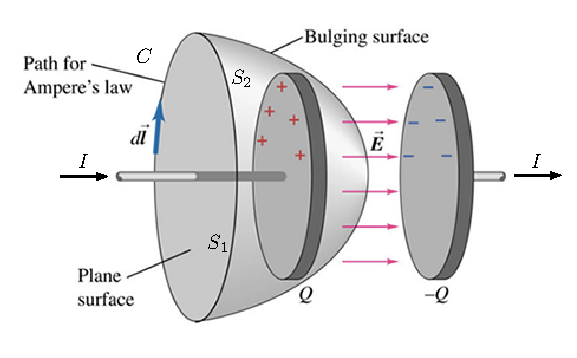
\includegraphics[height = 50mm, width=100mm, angle=0]{ampere.eps}.}
\caption{Inconsistency of Ampere's law for a charged capacitor, \cite{fig_7}}
\label{ampere.fig}
\end{figure}
Recall equation (\ref{steady_current.eqn}) from section \ref{mag_induction.sec}. Let the surfaces $S_1$ and $S_2$ correspond to the plane surface (disc) and the bulging surface (elliptic parabaloid), respectively. Let $C$ be the path that Ampere's law is applied to according to figure \ref{ampere.fig}. Applying Ampere's law for the magnetic intensity field from equation (\ref{induction1.eqn}) to each surface in figure \ref{ampere.fig} implies that
\begin{equation}
\oint_C\vec{H}\circ d\vec{l}=\int_{C}\vec{J}\circ\hat{n}\,da=I\quad\mbox{and}\quad\oint_{S_1}\vec{H}\circ d\vec{l}=\int_{S_2}\vec{J}\circ\hat{n}\,da=0.
\end{equation}
At this point in developing these equations for figure \ref{ampere.fig}, Ampere's law implies that $I=0$, but it is observed that a non-zero current is present in the wire. The electric field existing between the plates must be accounted for. 

The inconsistency in Ampere's law is resolved using the differential form of the law from equation (\ref{intensity_curl.eqn}). Observe that the divergence of any curl is necessarily zero for any vector field. This implies that the continuity equation for current density, given by (\ref{current_cont2.eqn}), is also inconsistent because steady current satisfies equation (\ref{current.eqn}). 

Recall the definition of Maxwell's first equation, (\ref{e_gauss_diff.eqn}), and apply this to the continuity equation to obtain
\begin{equation}
\vec{\nabla}\left[\vec{j}+\frac{\partial\vec{D}}{\partial t}\right]=0,
\end{equation}
for a sufficiently continuous displacement field, $\vec{D}$, as a function of space and time coordinates. Redefining Ampere's law as
\begin{equation}\vec{\nabla}\times\vec{H}=\vec{J}+\frac{\partial\vec{D}}{\partial t},
\label{maxwell4.eqn}
\end{equation}
removes the inconsistency and is the definition of Maxwell's fourth equation.
\subsection{Maxwell's Wave Equation}\label{maxwell_wave.sec}
Refer to \cite{Reitz} and \cite{Belanger} in this subsection. This subsection combines Maxwell's equations (\ref{maxwell1.eqn}), (\ref{maxwell2.eqn}), (\ref{maxwell3.eqn}) and (\ref{maxwell4.eqn}) to derive Maxwell's wave equation. 

The glass core of the optical fiber being considered is non-conductive by virtue of how it is defined in section \ref{properties.sec} to be isotropic, homogeneous, non-birefringent and lossless. This implies that the current density, $\vec{J}$, and charge density, $\rho$, is zero. In other words, the core is charge neutral with respect to Maxwell's equations and the transfer of charges within the core is unimpeded. Moreover, Maxwell's equations are independent of $\vec{J}$ and $\rho$ according to the derivations throughout section \ref{maxwellsequations}. Also note that the magnetization field, $\vec{M}$, is zero because charges embedded in the core are statically and dynamically neutral.

The first and fourth of Maxwell's equations reduce to
$$\vec{\nabla}\circ\vec{D}\qquad\mbox{and}\qquad\vec{\nabla}\times\vec{H}=\frac{\partial\vec{D}}{\partial t}.$$ Computing the curl of equation (\ref{maxwell3.eqn}) and (\ref{maxwell4.eqn}) obtains
\begin{equation}
\vec{\nabla}\times\vec{\nabla}\times\vec{E}=-mu_0\frac{\partial\vec{\nabla}\times\vec{D}}{\partial t}\qquad\mbox{and}\qquad\vec{\nabla}\times\vec{\nabla}\times\vec{H}=\frac{\partial\vec{\nabla}\times\vec{D}}{\partial t}.
\label{maxwell_wave1.eqn}
\end{equation}

It is necessary to rewrite the second wave equation with respect to $\vec{E}$ since $\vec{D}$ describes the charges embedded in the core, which behave neutrally. At the same time, the equation (\ref{displacement_field.eqn}) is applied to the equation on the right hand side of (\ref{maxwell_wave1.eqn}) to obtain
$$\vec{\nabla}\times\vec{\nabla}\times\vec{H}=\varepsilon\frac{\partial\vec{\nabla}\times\vec{E}}{\partial t}.$$

Observe that for any vector field, $\vec{A}$, the equation
$$\vec{\nabla}\times\vec{\nabla}\times\vec{A}=-\nabla^2\vec{A}+\vec{\nabla}\left(\vec{\nabla}\circ\vec{A}\right)$$
is satisfied by applying the definitions and theorems in appendix \ref{A.sec}. Applying this to the equations (\ref{maxwell_wave1.eqn}) gives
\begin{equation}
\nabla^2\vec{E}-\mu_0\varepsilon\frac{\partial^2\vec{E}}{\partial t^2}=\vec{\nabla}\left(\vec{\nabla}\circ\vec{E}\right)\qquad\mbox{and}\qquad\nabla^2\vec{H}+\varepsilon\frac{\partial^2\vec{H}}{\partial t^2}=\vec{\nabla}\left(\vec{\nabla}\circ\vec{H}\right)
\label{double_curl.eqn}
\end{equation}

From equation (\ref{maxwell1.eqn}) and (\ref{constitutive.eqn}), the dot product is directly applied to obtain
$$\vec{\nabla}\circ\vec{D}=\varepsilon\vec{\nabla}\circ\vec{E}+\varepsilon\vec{E}\circ\vec{\nabla}\varepsilon=0.$$ According to subsection \ref{displacement.sec}, $\varepsilon$ is a constant. Therefore, the gradient is zero, which implies that 
\begin{equation}
\vec{\nabla}\circ\vec{E}=0.
\label{electric_divergence.eqn}
\end{equation}
Applying (\ref{maxwell2.eqn}) and (\ref{electric_divergence.eqn}) to (\ref{double_curl.eqn}) gives Maxwell's wave equation with respect to either $\vec{E}$ or $\vec{H}$ and is defined by the equations
\begin{equation}
\nabla^2\vec{E}=\mu_0\varepsilon\frac{\partial^2\vec{E}}{\partial t^2}\qquad\mbox{and}\qquad\nabla^2\vec{H}=-\varepsilon\frac{\partial^2\vec{H}}{\partial t^2}.
\label{maxwell_wave.eqn}
\end{equation}
\section{The Second Order Wave Equation}
\subsection{Hyperbolic PDEs}\label{hyp.sec}
This section mainly follows \cite{Kev} and course notes in partial differential equations. The method of characteristics is used to define hyperbolic partial differential equations (PDEs). Refer to appendices \ref{DEs} and \ref{character.sec} for a discussion on PDEs and the method of characteristics, respectively. We restrict our attention to second order semi-linear PDEs with 4-independent variables, since this is the nature of Maxwell's wave equation. The motivation for defining hyperbolic second order PDEs is to define Maxwell's wave equation as a hyperbolic PDE and present an example of the general wave equation in 1-dimensional space. The example illustrates the existence of unique solutions for $1$-dimensional wave equation and what possible solutions may look like for light propagation in optical fibers. The example also illustrates a plane wave which is defined in subsection \ref{plane_waves.sec}

First, we define hyperbolic PDEs. The general wave equation which represents Maxwell's wave equation is discussed in subsection . Then, the method of characteristics is applied to the 1-dimensional wave equation.
\begin{definition}\textbf{(Hyperbolic PDE)}
In general, a PDE is defined as hyperbolic at particular sets of points in the domain, $\Omega$, of the solution. It is hyperbolic at points where the Cauchy problem for the PDE, (having a hyper-surface solution at the point of interest), has a unique solution in the neighbourhood of the point on any non-characteristic hyper-plane passing though the point. This definition is interpreted from the results in appendix \ref{character.sec}.
\end{definition}

Semi-linear PDEs are classified as hyperbolic according to the principal part of the PDE since it determines the dominant behaviour of changes in the hyper-surface solution.

\begin{definition}\textbf{(Restriction of Semi-Linear PDEs)}
We may write a second order semi-linear PDE with 4 independent variables in the form
\begin{multline}a_1(x,y,z,t)u_{xx}+a_2(x,y,z,t)u_{xy}+a_3(x,y,z,t)u_{xz}+a_4(x,y,z,t)u_{xt}\\+a_5(x,y,z,t)u_{yy}+a_6(x,y,z,t)u_{yz}+a_7(x,y,z,t)u_{yt}+a_8(x,y,z,t)u_{zz}\\+a_9(x,y,z,t)u_{zt}+a_{10}(x,y,z,t)u_{tt}+ b(x,y,z,t,u,u_x,u_y,u_z,u_t)=0.\nonumber
\end{multline}
The principal part of this semi-linear PDE is defined by
\begin{multline}a_1(x,y,z,t)u_{xx}+a_2(x,y,z,t)u_{xy}+a_3(x,y,z,t)u_{xz}+a_4(x,y,z,t)u_{xt}\\+a_5(x,y,z,t)u_{yy}+a_6(x,y,z,t)u_{yz}+a_7(x,y,z,t)u_{yt}+a_8(x,y,z,t)u_{zz}\\+a_9(x,y,z,t)u_{zt}+a_{10}(x,y,z,t)u_{tt}=0,\label{principal.eqn}
\end{multline}
and corresponds to the highest derivatives present in the PDE, in general. The method of characteristics is applied to the principal part of a semi-linear PDE.
\end{definition}

%\subsubsection*{(Effects of Cauchy Data on Existence and Uniqueness %of Solutions to PDEs)}
%Consider a first order quasi-linear PDE,
%$$a(x,y,u)u_x+b(x,y,u)u_y=c(x,y,z),$$
%with Cauchy data given on some curve $\Gamma$ given by the reference point determined by $x=x_0(\tau)$, $y=y_0$, $u_0(\tau)$. Assume that these are differentiable with respect to $\tau$. It follows by differentiating that,
%$$\frac{du_0}{d\tau}=\frac{\partial u}{\partial x}\frac{dx_0}{d\tau}+\frac{\partial u}{\partial y}\frac{dy_0}{d\tau},$$
%is satisfied. The PDE must also be satisfied on the curve $\Gamma$ and implies that
%$$c(x,y,u)=a(x,y,u)\frac{\partial u}{\partial x}+b(x,y,u)\frac{\partial u}{\partial y}.$$ This gives the following system of equations:
%\begin{equation}
%\left( \begin{array}{cc} a & b \\
%\frac{dx_0}{d\tau} & \frac{dy_0}{d\tau}\end{array} \right)
%\left( \begin{array}{c} u_x \\ u_y \end{array} \right)=\left( \begin{array}{c} c \\ \frac{du_o}{d\tau} \end{array} \right)
%\end{equation}
%Therefore, $u_x$ and $u_y$ are uniquely determined if the determinant of this system of equations is non-zero. If so, the solution surface is uniquely defined close to points of $\Gamma$ and
%$$\Delta=det\left( \begin{array}{cc} a & b \\
%\frac{dx_0}{d\tau} & \frac{dy_0}{d\tau}\end{array} \right)=a\frac{dy_0}{d\tau}-b\frac{dx_0}{d\tau}=0\quad\Leftrightarrow\quad(x'_0\big(\tau),y'_0(\tau)\big)\,\mbox{is parallel to}\,(a,b).$$
%The three possibilities for this determinant must be checked, such that $\Gamma$ is a characteristic. These possibilities are given by the following:
%\begin{enumerate}
%\item $\Delta\neq 0$ implies that $\Gamma$ is not a characteristic, since there is a unique solution to the PDE in a neigbourhood of $\Gamma$, but such a solution may fail to exist on the entire domain. In other words, characteristics may be intersecting, so we cannot guarantee a unique solution to the PDE on $\Gamma$, whenever solutions to the system of equations exist.
%\item If $\Delta=0$ and $\big(x'_0(\tau),y'_0(\tau)\big)=k(a,b)$ for some non-zero constant $k$ then $\Gamma$ is not a characteristic, since $\big(x'_0(\tau),y'_0(\tau)\big)$ is the tangent plane of the projection of $\Gamma$ in the $(x,y)$-plane and $(a,b)$ project characteristics in the $(x,y)$-plane. This corresponds to the system of equations having no solutions containing $\Gamma$.
%\item If $\Delta=0$, $\big(x'_0(\tau),y'_0(\tau)\big)=k(a,b)$ and $\big(x'_0(\tau),y'_0(\tau),u'_0(\tau)\big)=k(a,b,c)$ for some non-zero constant $k$, then there are infinitely many solutions to the system of equations. Infinite solutions implies that $\Gamma$ is exclusively and uniquely contained in the solution surface for any point $\tau$.
%\end{enumerate}
\subsection{Second Order Wave Equation}\label{wave.sec}
The wave equation is most generally a second order linear PDE. It may be defined in up to $n$-dimensions. The wave equation is referred to as an $(n-1)$-dimensional wave equation to account for spatial dimensions whenever it describes oscillatory phenomenon in time and space. Let $c$ be some constant and $(x,y,z,t)\in\Omega$ be the domain of the solution to the PDE for the 3-dimensional wave equation. Then it is defined by
\begin{equation}
u_{tt}(x,y,z,t)-c^2\nabla^2u(x,y,z,t)=0,
\label{order2wave.eqn}
\end{equation}
where $\nabla^2$ is the Laplacian, which satisfies
$$\nabla^2u=u_{xx}+u_{yy}+u_{zz}$$
for $(x,y,z)\in\mathbb{R}^3$. Assuming sufficient continuity given by the Lipschitz condition, seeking points in the wave equation that are hyperbolic is equivalent to finding a transformation with respect to the method of characteristics such that characteristics intersect the solution uniquely in $\Omega$.

The method of characteristics differs as the dimensions of of the wave equation increase. The characteristics for the $n$-dimensional wave equation are $n$-dimensional hyper-planes. This can be shown by a generalization of the method from section \ref{hyp.sec}, which shows this for the $3$-dimensional wave equation. The parametrization is found implicitly by analyzing initial and boundary conditions that are required to form a dispersive solution in section \ref{guides.sec}. The resulting characteristic equations describe light rays propagating in the core and depend on conditions at the core-cladding boundary.

\subsection{1-Dimensional Wave Equation}
As an example, consider the 1-dimensional wave equation,
\begin{equation}
u_{tt}(x,t)-c^2u_{xx}(x,t)=0,\qquad x\in[0,L]\subset\mathbb{R},\quad t\in[0,\infty)\subset\mathbb{R}
\label{1dim_wave.eqn}
\end{equation}
with initial conditions 
$$u(x,0)=f(x),\, u_t(x,0)=g(x)$$ and boundary conditions
$$u(0,t)=0,\,u(L,t)=0.$$

First we use the method of characteristics for a general second order semi-linear PDE with two independent variables, $(x,t)$. The results are applied to the $1$-dimensional wave equation in order to show it is hyperbolic for a particular transformation. In addition, it is shown that there exists a transformation that is independent of any initial or boundary conditions. Refer to appendix \ref{character.sec} for applying the method of characteristics. 

Define an arbitrary second order semi-linear PDE with two independent variables as
\begin{equation}
\mathcal{L}[u]=a(x,t)u_{xx}+b(x,t)u_{tt}+c(x,t)u_{xt}+\mbox{lower order terms}=0.
\label{principal1.eqn}
\end{equation}

Define the transformation $(x,t)\mapsto(\xi,\eta)$ and use the chain rule to substitute $U_{\xi\eta}$, $U_{\xi\xi}$, $U_{\eta\eta}$, $U_\xi$, $U_\eta$ and $U(\xi,\eta)=u(x,t)$ into the PDE given by equation (\ref{principal.eqn}). It follows that
\begin{multline}
\mathcal{L}[U]=(a\xi_x^2+b\xi_x\xi_t+c\xi^2_t)U_{\xi\xi}+(2a\xi_x\eta_x+b\xi_x\eta_t+b\xi_t\eta_x+2c\xi_x\eta_t)U_{\xi\eta}\\+(a\eta^2_x+b\eta_x\eta_t+\eta^2_t)U_{\eta\eta}+\mbox{lower order terms}=0
\end{multline}
Define,
\begin{align*}
a\xi_x^2+b\xi_x\xi_t+c\xi^2_t&=\alpha,\\
2a\xi_x\eta_x+b\xi_x\eta_t+b\xi_t\eta_x+2c\xi_x\eta_t&=\beta,\\
a\eta^2_x+b\eta_x\eta_t+\eta^2_t&=\gamma.
\end{align*}
Then, it follows that
$$\beta^2-4\alpha\gamma=(b^2-4ac)(\xi_x\eta_t-\xi_t\eta_x)^2,$$
where, $\xi_x\eta_t-\xi_t\eta_x$, is the Jacobian of the transformation. This Jacobian is necessarily non-zero and finite according to appendix \ref{character.sec}.

Moreover, the discriminant,
\begin{equation}
b^2-4ac,
\label{disc.eqn}
\end{equation}
of the PDE does not change sign after the transformation, $(x,t)\mapsto (\xi,\eta)$. This implies that, in general, the form in which the principle part of semi-linear equations are written is independent with respect to the sign of the discriminant. Consequently, we define and analyze points in the solution space for second order semi-linear PDEs independently based on the sign of the discriminant, (\ref{disc.eqn}). In particular, hyperbolic second order PDEs with 2 independent variables are those for which $b^2-4ac>0$.

Upon applying a transformation, the PDE may be rewritten by substituting the transformed variables directly into the PDE. These are called canonical forms. Using a particular choice of transformation, we may represent any principle part of a semi-linear PDE in exactly three ways, each corresponding to the sign of the discriminant. We may define a transformation satisfying
\begin{align}
\alpha=a\xi_x^2+b\xi_x\xi_y+c\xi_y^2=b\xi_x\xi_y&=0\label{trans2.eqn}\\
\gamma=a\eta_x^2+b\eta_x\eta_y+c\eta_y^2=b\eta_x\eta_y&=0\label{trans1.eqn}
\end{align}
If these are true, suppose $a$ and $c$ are not both zero then
\begin{gather}
a\left(\frac{\xi_x}{\xi_y}\right)^2+b\left(\frac{\xi_x}{\xi_y}\right)+c=0\nonumber\\a\left(\frac{\eta_x}{\eta_y}\right)^2+b\left(\frac{\eta_x}{\eta_y}\right)+c=0\nonumber\\
a+b\left(\frac{\eta_y}{\eta_x}\right)+c\left(\frac{\eta_y}{\eta_x}\right)^2=0\\ a+b\left(\frac{\xi_y}{\xi_x}\right)+c\left(\frac{\xi_y}{\xi_x}\right)^2=0\nonumber
\end{gather}

These contradict the assumption that $a,c$ not both zero. Then the transformation which satisfies (\ref{trans1.eqn}) and (\ref{trans2.eqn}) necessarily satisfies
$$\frac{\eta_x}{\eta_y}=\frac{-b\pm\sqrt{b^2-4ac}}{2a}\quad\mbox{or}\quad\frac{\xi_x}{\xi_y}=\frac{-b\pm\sqrt{b^2-4ac}}{2a}.$$ 
For a valid transformation, the variables $\xi$ and $\eta$ are independent. Without loss of generality choose
$$\frac{\eta_x}{\eta_y}=\frac{-b-\sqrt{b^2-4ac}}{2a}\quad\mbox{or}\quad\frac{\xi_x}{\xi_y}=\frac{-b+\sqrt{b^2-4ac}}{2a}.$$ Along a characteristic curve, one of the transformed variables are constant. Along a curve satisfying either $\xi(x,t)=\mbox{constant}$ or $\eta(x,t)=\mbox{constant}$, we obtain the differential equations
\begin{equation}
\frac{\partial\xi}{\partial x}+\frac{\partial\xi}{\partial y}\frac{dy}{dx}=0\quad\mbox{or}\quad\frac{\partial\eta}{\partial x}+\frac{\partial\eta}{\partial y}\frac{dy}{dx}=0,
\end{equation}
which imply that
\begin{equation}
\frac{dy}{dx}=-\frac{\xi_x}{\xi_y}=\frac{b-\sqrt{b^2-4ac}}{2a}\quad\mbox{or}\quad\frac{dy}{dx}=-\frac{\eta_x}{\eta_y}=\frac{b+\sqrt{b^2-4ac}}{2a}.
\label{1dim_char.eqn}
\end{equation}
Therefore, the transformation $(x,t)\mapsto(\xi,\eta)$ is defined by these relations and also defines all characteristic curves for the PDE.

This transformation is now applied to the $1$-dimensional wave equation from (\ref{1dim_wave.eqn}). From the $1$-dimensional wave equation it follows that $$a(x,t)=-c^2,\quad b(x,t)=0,\quad c(x,t)=1.$$ Then the equation is completely hyperbolic since $b^2-4ac=4c^2>0$. The characteristic equations defining the characteristic curves follow from  equations (\ref{1dim_char.eqn}) and the values of $a,b,c$, where
\begin{equation}
\frac{dt}{dx}=\frac{1}{c},\quad\mbox{or},\quad
\frac{dt}{dx}=\frac{-1}{c},
\end{equation}
implies that
\begin{equation}
x-ct=\eta(x,t)\qquad\mbox{and}\qquad x+ct=\xi(x,t)\label{1dim_trans.eqn}
\end{equation}
are the two families of characteristic curves that describe the solution. 
\subsection{Plane Waves}\label{plane_waves.sec}
A plane wave solution, known as the d'Alembert solution, is now derived for the $1$-dimensional wave equation. The plane wave is defined after the example involving the d'Alembert solution. The canonical form for the $1$-dimensional wave equation gives a plane wave solution by substituting transformations (\ref{1dim_trans.eqn}) into the wave equation. It follows that $\xi_x=1,\,\,\xi_t=c,\,\,\eta_x=1$ and $\,\,\eta_t=-c$ which implies
\begin{gather}
u_{tt}=c^2\left(\frac{\partial}{\partial\xi}-\frac{\partial}{\partial\eta}\right)^2U=c^2U_{\xi\xi}-2U_\xi U_\eta-U_{\eta\eta}\nonumber\\
u_{xx}=\left(\frac{\partial}{\partial\xi}+\frac{\partial}{\partial\eta}\right)^2 U=c^2 U_{\xi\xi}+2U_\xi U_\eta+U_{\eta\eta}
\end{gather}
by applying the chain rule several times.

Inputting these into the $1$-dimensional wave equation gives $-4c^2U_{\xi\eta}$. Integrating this directly gives
\begin{equation}
u(x,t)=p(x+ct)-q(x-ct)=
\label{canonsol.eqn}
\end{equation}
for some functions $p$ and $q$. We may write $u_t=cp'-cq'$ and apply the initial conditions $u_t(x,0)=g(x)$ and treat this as an initial value problem independent of the boundary conditions, $u(0,t)=0$ and $u(L,t)=0$. The result is
\begin{align*}
p'(x)=\frac{1}{2c}\left(g(x)+cf'(x)\right)&\Rightarrow p(x)=\frac{1}{2}f(x)+\frac{1}{2c}\int_0^x g(s)ds+c_0,\quad c_0=\mbox{const.}\\&\Rightarrow p(x+ct)=\frac{1}{2}f(x+ct)+\frac{1}{2c}\int_0^{x+ct}g(s)ds +c_0.
\end{align*}
Similarly,
$$q(x-ct)=\frac{1}{2}f(x-ct)-\frac{1}{2c}\int_0^{x-ct}g(s)ds -c_0.$$ Inputting these into the solution from (\ref{canonsol.eqn}) gives the d'Alembert solution
\begin{align*}
u(x,t)&=\frac{1}{2}\Big(f(x+ct)+f(x-ct)\Big)+\frac{1}{2c}\left[\int_0^{x+ct}g(s)ds-\int_0^{x-ct}g(s)ds\right]\\
&=\frac{1}{2}\Big(f(x+ct)+f(x-ct)\Big)+\frac{1}{2c}\int_{x-ct}^{x+ct}g(s)ds
\end{align*}

The boundary conditions $u(0,t)=0$ and $u(L,t)=0$ allows us to determine the solution at every point in $\Omega$ using the transformation $(x,t)\mapsto(\xi,\eta)$. In general, by choosing any constants $(\eta_0,0)$ and $(\xi,0)$, the hyperbolic region bounded by non-intersecting characteristics is illustrated in figure {\ref{figure_IBVP1} as the green region. This is called the domain of influence.

Solutions are defined along either of the characteristic lines $\eta=x-ct$ and $\xi=x+ct$ for any $\xi,\eta\in(\eta_0,\xi_0)\subset\mathbb{R}$. The solution is unique in the domain of influence by the method of characteristics, since neither characteristics intersect there.

The domain of dependence is defined as the interval that initial conditions are given on. In general this may be a set rather than an interval. Conditions at this boundary completely determine the behaviour of the solution in the domain of influence. This is valid for any pair of points $(\eta_0,0)$ and $(\xi_0,0)$ in the initial value problem.
\begin{figure}[h!]
\centerline{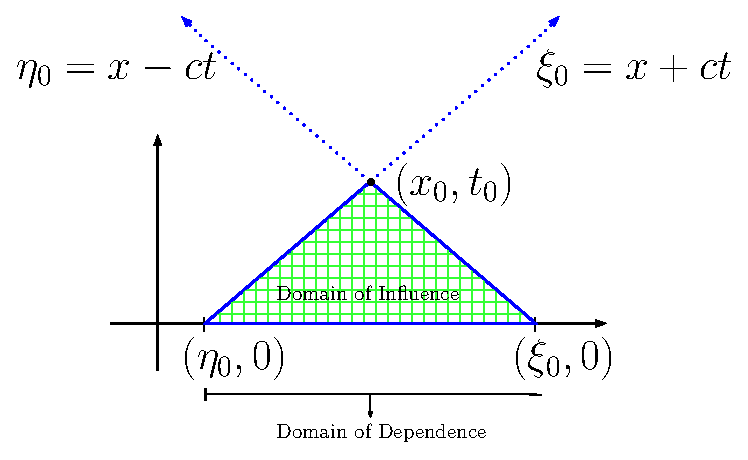
\includegraphics[height = 50mm, width=60mm, angle=0]{IBVP1.eps}}
\caption{Region for the d'Alembert solution.}
\label{figure_IBVP1}
\end{figure}

Now we may apply the boundary conditions $$u(0,t)=0,\, u(L,t)=0.$$
This restricts the initial value problem to a fixed domain of dependence of length $L$, but the characteristic equations do not change. The result is shown in figure \ref{figure_IBVP2}.

The domain of dependence is now the interval $(0,L)$. The d'Alembert solution may be integrated over the region bounded by any unique non-intersecting characteristic lines to find the solution there. By defining the odd periodic extensions of $f(x)=\bar{f}(x)$ and $\bar{g}(x)$ on the interval $(-L,L)$, we may write the d'Alembert solution as
\begin{equation}
u(x,t)=\frac{1}{2}\Big(\bar{f}(x+ct)+\bar{f}(x-ct)\Big)+\int_{x-ct}^{x+ct}\bar{g}(s)ds.
\end{equation}

Doing this allows pairs of characteristics to be defined arbitrarily and the d'Alembert solution is transformed along the corresponding domain of influence to give solutions at those points. This is done canonically to define the solution at any point in the column illustrated in the figure.
\begin{figure}[h!]
\centerline{\includegraphics[height = 80mm, width=180mm, angle=0]{IBVP2.eps}}
\caption{Solution to IBVP for the $1$-dimensional wave equation.}
\label{figure_IBVP2}
\end{figure}

This is valid for any $0<x<L$ and any $t>0$. Moreover, we may visualize the characteristics behaving like reflections between the boundaries $u(0,t)=0$ and $u(L,t)=0$. The solution at any point on the dashed blue line is determined entirely by the domain of dependence, (highlighted yellow), and the characteristic lines. In other words, characteristic lines are independent of the placement of the boundary conditions $u(0,t)=0$ and $u(L,t)=0$. The boundary conditions are only indicating where the solution is bounded on the $x$-axis and what its value is on that boundary.

The d'Alembert solution to the IBVP for the $1$-dimensional wave equation is called a plane wave solution. The planes being referred to in the example here are defined by the lines $x+ct$ and $x-ct$. It turns out that for the $1$-dimensional wave equation example, these are points rather than planes. In general, plane wave solutions represent a type of solution for PDEs with arbitrarily many independent variables.

Plane waves are functions describing oscillations in space and time. In general, a plane wave solution to a hyperbolic PDE may be written as
$$u(x_1,...,x_n,t)=f\left(a \vec{x}-bt\right),$$
for position $\vec{x}$ and time $t$.
Let $c$ be a constant. For a value of the solution $u( \vec{x}_0,t_0)=c$, the plane
$$a\vec{x}_0-bt=c$$
propagates its points with a speed $a\slash b$ at any given moment in time. This is developed further when defining dispersion in section \ref{wavesintro.sec}. Plane wave solutions propagate in the domain of influence based entirely on the conditions placed on a domain of dependence from which the plane wave originates.

We seek solutions of this form for Maxwell's wave equation. In an optical fiber, a plane wave solution corresponds to oscillatory solutions in the core determined strictly by the initial beam of light entering the core through one of its circular faces and by characteristic equations. The characteristic equations are independent of the core-cladding boundary conditions since rays of light are parametrized and form characteristics.
\section{Dispersion}
\subsection{Introduction to Dispersive Waves}\label{wavesintro.sec}
In this section, the notion of dispersion is introduced, following \cite{Whitham}. Refer to the definitions in appendix \ref{DEs} and consider a PDE given by semi-linear differential operator $\mathcal{L}[\varphi]$, with solution $u$. Note that in this introductory subsection one dimension of space is assumed, but in general, multiple dimesions of space may occur and are considered in the subsections which follow here.

The solution, $\varphi$, is dispersive whenever it is an oscillatory solution of the form,
\begin{equation}
\varphi= a\,cos(\kappa x - \omega t),
\label{gen_disp_solution.eqn}
\end{equation}
where the frequency, $\omega$, is a real function of the wavenumber, $\kappa$, and the function $\omega(\kappa)$ is determined from the particular PDE being considered. Note that this is a plane wave solution.

When solutions to a PDE are dispersive, the dispersion is characterized by the propagation of wavenumbers. The phase speed in the oscillatory solution, (\ref{gen_disp_solution.eqn}) is given by
$$\frac{\omega(\kappa)}{\kappa}.$$
The solution is said to be dispersive if this phase speed is not a constant and depends on $\kappa$. The term dispersion refers to the fact that a more general solution consists of the superposition of more than one oscillatory solution, like (\ref{gen_disp_solution.eqn}), each corresponding to different possible values of $\kappa$. This implies that different modes, (corresponding to possible values of $\kappa$), may propagate the respective wavenumbers, (determined by $\kappa$), with a different velocity. Plane wave solutions \textit{may} exist when they are oscillatory and could be `changing' with respect to time according to the dispersion. The plane wave solution is discussed further in section \ref{guides.sec}.

First, in subsection \ref{dispersion.sec}, the dispersion is defined with respect to linear PDEs. In subsection \ref{groupvelocity}, the notion of group velocity is defined and corresponds to the possibly varying phase velocities of frequency modes $\omega(\kappa)$.
\subsection{Linear Dispersive Waves}\label{dispersion.sec}
This section defines dispersion, so that we may find possible dispersive solutions to Maxwell's wave equation following \cite{Whitham}. The classification of dispersive waves is made on the type of solution rather than on the differential equation. Let $A$ be a complex constant. Let $\omega$ be a real constant. Let $\vec{\kappa}$ and $\vec{x}$ be real valued vectors in cylindrical coordinates, where $\vec{\kappa}$ is constant. Dispersive waves are recognized by wave train solutions of the form
\begin{equation}
\phi (\vec{x},t)=Ae^{i\vec{\kappa}\circ\vec{x}-i\omega t}.
\label{generalsolution.eqn}
\end{equation}

Suppose such a solution needs to satisfy a \textit{linear} partial differential equation in cylindrical coordinates. The differential equation gives a relation 
\begin{center}
$F\bigg(r, \theta , z, t, \phi , \frac{\partial\phi}{\partial r}, \frac{\partial\phi}{\partial\theta}, \frac{\partial\phi}{\partial z}, \frac{\partial\phi}{\partial t}, \frac{\partial^2\phi}{\partial r\partial\theta}, \frac{\partial^2\phi}{\partial r\partial z},\frac{\partial^2\phi}{\partial r\partial t}, \frac{\partial^2\phi}{\partial\theta\partial z}, \frac{\partial^2\phi}{\partial\theta\partial t}, \frac{\partial^2\phi}{\partial z \partial t}, \frac{\partial^2\phi}{\partial r^2}, \frac{\partial^2\phi}{\partial\theta^2}, \frac{\partial^2\phi}{\partial z^2}, \frac{\partial^2\phi}{\partial t^2}\bigg)=0,$
\end{center}
which is a linear function of $\phi(\vec{x},t)$ and its partial derivatives. Note that $\phi(\vec{x},t)$ is separable with respect to $x_r,x_\theta,x_z,t$ since $\vec{\kappa}\circ\vec{x}$ is a linear combination of $x_r,x_\theta,x_z$. This implies that mixed partial derivatives are equal in $F$. Taking partial derivatives with respect to either $t$ or $\vec{x}$ will produce factors of either $\omega$ or simultaneously $x_r,x_\theta,x_z$, respectively.

The relation $F(\vec{*})=0$ reduces to 
\begin{equation}
G(\omega,\kappa_r,\kappa_\theta,\kappa_z)=0
\label{disprel1.eqn}
\end{equation}
by factoring out $\phi (\vec{x},t)$. By construction of $G$, it is a linear equation with respect to $\omega,\kappa_r,\kappa_\theta,\kappa_z$ and is called the dispersion relation. The roots of $G$ with respect to $\omega$ are given by relations
$$\omega_j=W_j(\vec{\kappa})=W_j(\kappa_r,\kappa_\theta,\kappa_z),$$
where $\omega_j$ is a distinct root with corresponding relation $W_j$.

Let $\omega$ represent an arbitrary root $\omega_j$. To obtain real solutions,
\begin{equation}
Re(\phi)=\vert A\vert\cos (\vec{\kappa}\circ\vec{x}-\omega t+arg\,A)=\varphi
\label{genrealsol.eqn}
\end{equation}
is an oscillatory wave with respect to time and space. Let $\vartheta=\vec{\kappa}\circ\vec{x}-\omega t$, where $\vec{x}=x_1\hat{r}+x_2\hat{\theta}+x_3\hat{z}$ is the position of a point in 3-dimensional cylindrical coordinate space. Then $\vartheta$ accounts for any change in spatial position with respect to time in $\varphi$ as it oscillates, since $arg\,A$ is constant. By definition, the variable $\vartheta$ is the phase of $\varphi$. Fixing $\vartheta=$ constant defines a spatial plane that changes with respect to time. These are called phase surfaces.

Next, the oscillatory behaviour of $\varphi$ in the spatial and temporal contexts with respect to phase surfaces will be considered. This makes sense because we may separate $Re(\phi)$ as a product of a time dependent oscillatory functions and spatially dependent oscillatory functions by using the multiplicative properties of the exponential function prior to taking the real part.

When dealing with spatial oscillations in radial units, we refer to one cycle of the wave as its wavelength and the number of cycles per $2\pi$ degrees as its wavenumber. Similarly, one cycle of a temporal wave is the period and the number of cycles per $2\pi$ radians is the frequency. The spatial gradient of a phase surface is the gradient of the plane
$$\vartheta\vert_{t=0}=\text{constant},$$
for some constant.

For any constant defining a phase surface and any fixed point in time, the points of the surface are linearly shifted by the constant and the time dependent part of $\vartheta$. Therefore, the position of an arbitrary point of the surface for some instant in time is determined by $\vec{\kappa}\circ\vec{x}=C$ for any constant $C$. Hence, we may equivalently let $C=0$ to define the position of points for any phase surface at an instant in time for some dispersion mode, $\omega$. The spatial gradient of the plane $\vartheta=C$ is given by the vector $\vec{\kappa}$ by definition of the gradient for the plane $\vec{\kappa}\circ\vec{x}=0$ and by observing it is the same for any constant $C$. Therefore, the spatial gradient of $\vartheta$ is always $\vec{\kappa}$ and has magnitude $\kappa=\vert\vec{\kappa}\vert$ for some dispersion mode $\omega$. Similarly, we may take the gradient with respect to $t$. The gradient simplifies as $\vartheta_t$. By construction of $\vec{\nabla}\vartheta$ and by definition of the gradient, $\kappa$ is the average number of crests for $\varphi$ per 3-dimensional unit distance.

Also, $-\vartheta_t$ is the average number of crests in the real solution, $\varphi$, per unit time in the direction of $\kappa$. Using radial units we may define the wavenumber and frequency of a phase surface to be $\kappa$ and $\omega$ respectively. Moreover, we may define wavelength and period as $\lambda=2\pi\slash\kappa$ and $\tau=2\pi\slash\omega$ respectively. In conclusion, each wavenumber $\omega$ has a continuum of phase surfaces $\vartheta=$ constant.

Consider the velocity of an arbitrary 3-dimensional point on a phase surface, $\vartheta=C$, for any constant $C$. The velocity of such a point is \textit{in the direction that is perpendicular to the phase surface} and has a \textit{magnitude} of wavelength per period given by $\omega\slash\kappa$. Therefore, the phase velocity is defined as
$$\vec{c}=\frac{\omega}{\kappa}\hat{\kappa},$$
where $\hat{\kappa}=\vec{\kappa}\slash\kappa$ is the unit vector  in the direction of $\vec{\kappa}$. Note that the phase velocity only accounts for the spatial variation in the phase surfaces with respect to time in the direction of $\hat{\kappa}$ for a particular frequency mode $\omega$.

In \cite{Whitham}, the author restricts the definition of dispersion to accommodate the following two cases. The first case may be observed by the heat equation $\varphi_t=\nabla^2\varphi$ giving complex modes of dispersion of the form $\omega=-i\kappa^2$ when a solution of the form (\ref{generalsolution.eqn}) is applied. It follows that the real part of the solution becomes $$Re(\varphi)=\kappa\vert A\vert\cos(\vec{\kappa}\circ\vec{x}+ arg\,A)$$ which is oscillatory only with respect to space. To maintain wavelike solutions in the first case, the class of linear dispersion is restricted to equations with dispersion relations that have only real solutions. This is equivalent to the restriction
$$W(\vec{\kappa})\neq 0.$$

The second case is observed whenever the group velocity is constant. The group velocity is defined in section \ref{groupvelocity}. The restriction for the second case is only stated here and the justification can be deduced from the arguments in section \ref{groupvelocity}. The second restriction is
\begin{equation}
det\left|\frac{\partial^2 W}{\partial\kappa_i\partial\kappa_j}\right|\neq 0.
\label{restriction2.eqn}
\end{equation}

One may also refer to section 11.1 of \cite{Whitham} to see the correspondence between the dispersion relation and their \textit{linear} differential equations is one-to-one. This means that one may be obtained from the other and vice versa. Therefore, the properties derived from a linear dispersive relation correspond uniquely to a linear differential equation and vice versa.
\subsection{Group Velocity for Linear PDEs}
\label{groupvelocity}
This subsection also follows \cite{Whitham}. We define the group velocity because a solution can only be dispersive if it admits group velocity behaviour. The group velocity behaviour may possibly be trivial for the simplest cases of a dispersive solution, which is shown in section \ref{guides.sec}.

First, the group velocity is derived in 1-dimensional space and then extended to 3-dimensional space. Recall the solution of the form of equation (5.2) with real part as in (5.4) such that one dimension of space is assumed. Assume a phase function $\vartheta(x_1,t)$ exists and describes the \textit{local} action of points in a phase surface with respect to time. By local, this means at the level of continuous dependence of the phase $\vartheta$ on points, $x_1$, and time, $t$.

The local wavenumber and local frequency are defined by
\begin{equation}
\kappa=\vartheta_{x_1}
\label{localphase1.eqn}
\end{equation}
and
\begin{equation}
\omega=-\vartheta_t.
\label{localphase2.eqn}
\end{equation}
Let an arbitrary dispersion relation corresponding to a linear differential equation exist. Let the corresponding dispersion relation be given as
$$\omega=W(\kappa).$$

Now we determine an equation that allows us to solve for $\kappa(x,t)$. It follows from differentiating (\ref{localphase1.eqn}) and (\ref{localphase2.eqn}) that $$\frac{\partial\kappa}{\partial t}=\vartheta_{x_1 t}$$ and $$\frac{\partial\omega}{\partial x_1}=-\vartheta_{tx_1},$$ where mixed partial derivatives are equal.
\begin{equation}
\frac{\partial\kappa}{\partial t}+\frac{\partial\omega}{\partial x_1}=\frac{\partial\kappa}{\partial t}+\frac{\partial W(\kappa)}{\partial x_1}=\frac{\partial\kappa}{\partial t}+\frac{dW(\kappa)}{d\kappa}\frac{\partial\kappa}{\partial x_1}=0,
\label{nonlinearwave.eqn}
\end{equation}
where
$$C(\kappa)=W'(\kappa)$$
is the propagation velocity of the wavenumber $\kappa(x_1,t)$. This propagation velocity defines the group velocity. Equation (\ref{nonlinearwave.eqn}) is a non-linear version of the simple wave equation. Now the group velocity is extended to the case of 3-dimensional space in cylindrical coordinates. The assumed phase function becomes a function $\vartheta(x_1,x_2,x_3,t)$, where $\vec{x}=x_1\,\hat{r}+x_2\,\hat{\theta}+x_3\,\hat{z}$. The local frequency $\omega$ and local wavenumber $\vec{\kappa}=\kappa_1\,\hat{r}+\kappa_2\,\hat{\theta}+\kappa_3\,\hat{z}$ are defined by
\begin{equation}
\omega=-\frac{\partial\vartheta}{\partial t}
\label{groupvelocity1.eqn}
\end{equation}
and
$$\kappa_i=\frac{\partial\vartheta}{\partial x_i},$$
for $i=1,2,3$. In the case of 3-dimensional space, the dispersion relation for some linear differential equation becomes
$$\omega=W(\kappa_1,\kappa_2,\kappa_3,x_1,x_2,x_3,t).$$Although, different dispersion modes may have different group velocities and phase speeds, a mode itself is dispersive only if $W$ is a nonlinear function of $\vec{k}_j$.

Following a similar argument as for the 1-dimensional case, we may differentiate $\omega$ with respect to $x_1,x_2,x_3$ and differentiate $k_i$ with respect to $k_j$, for $i,j\,\epsilon\,\{ 1,2,3\}$ and $i\neq j$. For each $i\,\epsilon\,\{1,2,3\}$ we obtain a pair of equations
\begin{equation}
\frac{\partial\kappa_i}{\partial t}+\frac{\partial\omega}{\partial x_i}=0
\label{groupvelocity2.eqn}
\end{equation}
and
\begin{equation}
\frac{\partial\kappa_i}{\partial x_j}-\frac{\partial\kappa_j}{\partial x_i}=0
\label{groupvelocity3.eqn}
\end{equation}
for any $j\,\epsilon\,\{1,2,3\,\vert\, i\neq j\}$. Combining (\ref{groupvelocity1.eqn}) and (\ref{groupvelocity2.eqn}) gives
$$\frac{\partial\kappa_i}{\partial t} + \frac{\partial W}{\partial x_i}=0=\frac{\partial\kappa_i}{\partial t} + \frac{\partial W}{\partial\kappa_j}\frac{\partial\kappa_j}{\partial x_i}+\frac{\partial W}{\partial x_i},$$
for any $i\neq j$. This may be written as
$$\frac{\partial\kappa_i}{\partial t} + \frac{\partial W}{\partial\kappa_j}\frac{\partial\kappa_j}{\partial x_i}=-\frac{\partial W}{\partial x_i}$$
and (\ref{groupvelocity3.eqn}) may be applied to obtain
\begin{equation}
\frac{\partial\kappa_i}{\partial t} + \frac{\partial W}{\partial\kappa_i}\frac{\partial\kappa_j}{\partial x_i}=-\frac{\partial W}{\partial x_i}.
\label{groupvelocity4.eqn}
\end{equation}
In 3-dimensional space, group velocity is defined by determining $\vec{\kappa}$ using equation (\ref{groupvelocity4.eqn}) for each $i\,\epsilon\,\{1,2,3\}$. In doing so, the components
$$C_j(\kappa_1,\kappa_2,\kappa_3,x_1,x_2,x_3,t)=\frac{\partial W(\kappa_1,\kappa_2,\kappa_3,x_1,x_2,x_3,t)}{\partial\kappa_j}$$
define the group velocity $\vec{C}$. Solutions are dispersive only if the group velocity is not the same as the phase velocity, i.e. $\vec{c}\neq\vec{C}$.
%\subsubsection*{Justifying Second Condition for Definition of Dispersion}
%Recall the second restriction on the definition of dispersion given by (\ref{restriction2.eqn}). Without this restriction the group velocity is constant. A constant group velocity implies that modes do not disperse, i.e. phase surfaces remain constant for any time, $t$. Therefore, the restriction is necessary to define dispersion explicitly.
\section{Guided Modes in Cylindrical Waveguides}\label{guides.sec}
\subsection{Guided Rays of Light and Dispersion}\label{lightrays.sec}
This section is dedicated to finding the characteristic equations describing the distribution of light rays propagating through the core of an optical fiber. This section mainly follows \cite{Belanger}, \cite{Okamoto} and \cite{Agrawal} in order of most to least relevant according to the arguments presented here. Recall the discussion of light ray propagation from section \ref{properties.sec}.

In general, a guided mode refers to a particular dispersive solution governing the paths of light rays propagating along phase surfaces. In other words, a mode describes a particular path that a ray or families of rays may take. The dispersion modes described in section \ref{dispersion.sec} correspond to a whole range of light ray modes such that groups of light rays may belong to the same phase surface and propagate with a group velocity. 

Suppose a beam of light is coupled to the circular face of the optical fiber and is the domain of dependence for a plane wave solution. The possible dispersive solutions to the wave equation inside the core are found by tracing the paths of individual rays of light. By parametrizing rays of light, the initial and boundary conditions required for producing valid characteristic equations can be found. These characteristics, which describe the paths of each individual ray of light, form a unique dispersive solution based only on the light entering at the domain of dependence. The domain of dependence is the circular face of the core where light enters in the form of rays at any angle smaller than the acceptance angle.

We assume small distances and consequently short periods of time in order to make the assumption of linearity. The short distance assumption is required because the non-linearity is inherent of the material and occurs over long distances as solutions on the paths of light rays `disperse'. It is inherited by the dependence of the relative permittivity on frequency, where the assumption of linearity was made in section 3.2. Therefore, non-linearity cannot be neglected over long distances and so the assumption of short distances is required. 
\subsection{Characteristic Equations for Guided Modes}\label{modes.sec}
This subsection derives the characteristic equations that correspond to the paths of light rays. We continue to follow \cite{Okamoto} and \cite{Belanger}. In the case of linear dispersive waves, it is possible to work with uniform plane wave solutions and derive boundary conditions at the core-cladding interface satisfying a particular dispersive solution with respect to planar phase surfaces. We assume the solution is separable with respect to coordinates $r$, $\theta$, $z$ and $t$.

Monochromatic waves are defined as those which have all fields $\vec{E}$, $\vec{B}$, $\vec{D}$, $\vec{H}$, $\vec{P}$ and $\vec{M}$ characterized by a single frequency $\omega$. Monochromatic waves are represented in cylindrical coordinates by dispersive solutions of the form
\begin{equation}
\vec{E}(r,\theta,z,t)=\vec{E}(r,\theta,z)e^{-i\omega t}\qquad\mbox{and}\qquad\vec{H}(r,\theta,z,t)=\vec{H}(r,\theta,z)e^{-i\omega t}\nonumber
\label{monochromatic.eqn}
\end{equation}
whenever the time dependence of the field is taken as $e^{-i\omega t}$. Monochromatic waves are assumed so that dispersive solutions may be found whenever such solutions exist for a single frequency of light. In general, many frequencies can occur when multiple sources of light are present, but we consider the case of one source representing a monochromatic wave.  

Assuming that the wave in the core is monochromatic, the solutions from (\ref{monochromatic.eqn}) are inputted into Maxwell's third and fourth equations (\ref{maxwell3.eqn}) and (\ref{maxwell4.eqn}), respectively. Then, 
\begin{equation}
\vec{\nabla}\times\vec{E}=-\mu_0\frac{\partial\vec{H}}{\partial t}\qquad\mbox{and}\qquad\vec{\nabla}\times\vec{H}=\varepsilon\frac{\partial\vec{E}}{\partial t},\label{oscillatory_solution.eqn}
\end{equation}
where $\varepsilon=\varepsilon_0n^2$ for the refractive index, $n$.

The mean Poynting vector is derived in \cite{Belanger} and is shown there to be along the $z$-axis for electric and magnetic fields that are polarized perpendicularly to it along the $(r,\theta)$-plane. It represents the direction in which electromagnetic waves propagate when the electric and magnetic fields are polarized along the transverse directions $r$ and $\theta$.

The following derivation uses the assumption that the light is polarizable in these directions in order to assume plane wave solutions to Maxwell's wave equation of the form
\begin{equation}
\begin{array}{lcr}
\vec{E}(r,\theta,z,t)=\vec{E}(r,\theta)e^{i(\omega t-\beta z)}&\mbox{and}&\vec{E}(r,\theta,z,t)=\vec{H}(r,\theta)e^{i(\omega t-\beta z)}
\end{array}.\label{solutions.eqn}
\end{equation}

We now follow the arguments from \cite{Belanger}, \cite{Okamoto} and \cite{Agrawal} to find the characteristic equations describing the modal distribution of light rays. These are exactly the characteristic equations that correspond to the dispersive solutions within the core satisfying prescribed boundary conditions. The use of boundary conditions for interpreting group velocity behaviour of solutions is shown at the end of this section. The validity of solutions is also discussed further in this section.

The cylindrical component version of the gradient, derived in appendix \ref{C.app}, must be applied to the equations (\ref{oscillatory_solution.eqn}). In the following derivations, the details related to the first equation from (\ref{oscillatory_solution.eqn}) are shown and results related to the second equation from (\ref{oscillatory_solution.eqn}) are stated, since they are similar and can be found in \cite{Belanger} and \cite{Okamoto}. Applying the cylindrical gradient gives
\begin{multline}
\quad\quad\,\vec{\nabla}\times\vec{E}e^{i(\omega t-\beta z)} = \bigg[\frac{1}{r}\frac{\partial\vec{e}_{z}(t)}{\partial\theta}-\frac{\partial\vec{e}_{\theta}(t)}{\partial z}\bigg]\hat{r}+\bigg[\frac{\partial\vec{e}_{r}(t)}{\partial z}-\frac{\partial\vec{e}_{z}(t)}{\partial r}\bigg]\hat{\theta}\\
+\bigg[\frac{1}{r}\frac{\partial\vec{e}_{r}(t)}{\partial\theta}+\frac{\vec{e}_{\theta}(t)}{r}-\frac{\partial\vec{e}_{\theta}(t)}{\partial r}\bigg]\hat{z}\\
=\bigg[\frac{1}{r}\frac{\partial E_z}{\partial\theta}e^{i(\omega t-\beta z)}+i\beta\frac{\partial E_{\theta}}{\partial z}e^{i(\omega t-\beta z)}\bigg]\hat{r}\\
\qquad\quad\, +\bigg[-i\beta\frac{\partial E_r}{\partial z}e^{i(\omega t-\beta z)}-\frac{\partial E_z}{\partial r}e^{i(\omega t-\beta z)}\bigg]\hat{\theta}\\
\,\,\quad+\bigg[\frac{1}{r}\frac{\partial E_r}{\partial\theta}e^{i(\omega t-\beta z)}+\frac{E_{\theta}}{r}e^{i(\omega t-\beta z)}-\frac{\partial E_{\theta}}{\partial r}e^{i(\omega t-\beta z)}\bigg]\hat{z}
\label{guides1.eqn}
\end{multline}
\begin{multline}
-\mu\frac{\partial\vec{h}(t)}{\partial t}=-\mu\frac{\partial\big(\vec{H}e^{i(\omega t-\beta z)}\big)}{\partial t}=-\mu\bigg[ i\omega H_{r}e^{i(\omega t-\beta z)}\bigg]\hat{r}-\mu\bigg[i\omega H_{\theta}e^{i(\omega t-\beta z)}\bigg]\hat{\theta}\\
-\mu\bigg[ i\omega H_{z}e^{i(\omega t-\beta z)}\bigg]\hat{z}\label{guides2.eqn}
\end{multline}
Observe that $\partial E_\theta\slash\partial z=E_\theta$ and $\partial E_r\slash\partial z=E_r$, since propagation is assumed in the $z$ direction. Also, observe by the chain rule that
$$\frac{E_\theta}{r}-\frac{\partial E_\theta}{\partial r}=\frac{1}{r}\left(\frac{\partial (rE_{\theta})}{\partial r} -\frac{\partial E_r}{\partial\theta}\right)$$

By applying these last two observations, factoring out $e^{i(\omega t-\beta z)}$ and equating the components in equations (\ref{guides1.eqn}) and (\ref{guides2.eqn}) we obtain the equations
\begin{gather}
\frac{1}{r}\frac{\partial E_z}{\partial\theta}+i\beta\frac{\partial E_{\theta}}{\partial z}=\frac{1}{r}\frac{\partial E_z}{\partial\theta}+i\beta E_{\theta}=-\mu_{0} i\omega H_r,\nonumber\\
-i\beta\frac{\partial E_r}{\partial z}-\frac{\partial E_z}{\partial r}=-i\beta E_r -\frac{\partial E_z}{\partial r}=-\mu_{0} i\omega H_{\theta},\label{guides3.eqn}\\
\frac{\partial E_{\theta}}{\partial r}+\frac{E_{\theta}}{r}-\frac{1}{r}\frac{\partial E_r}{\partial\theta}= \frac{1}{r}\left(\frac{\partial (rE_{\theta})}{\partial r} -\frac{\partial E_r}{\partial\theta}\right)=-\mu_{0} i\omega H_z.\nonumber
\end{gather}

A similar procedure is followed for the curl corresponding to the second equation from (\ref{oscillatory_solution.eqn}) and results in the equations
\begin{gather}
\frac{1}{r}\frac{\partial H_z}{\partial\theta}+i\beta H_{\theta}=i\varepsilon_{0}\omega n^2 E_r,\nonumber\\
-i\beta H_r -\frac{\partial H_z}{\partial r}=i\varepsilon_{0}\omega n^2 E_{\theta},\label{guides4.eqn}\\
\frac{1}{r}\bigg(\frac{\partial (rH_{\theta})}{\partial r} -\frac{\partial H_r}{\partial\theta}\bigg)=i\varepsilon_{0}\omega n^2 E_z.\nonumber
\end{gather}

The boundary conditions for Maxwell's wave equations are such that the respective electric and magnetic fields are continuous at the core-cladding boundary. In other words, the tangential components of the electric and magnetic fields are equal between boundaries. In mathematical terms this means
\begin{equation}
\begin{array}{cccc}
E_{t}^{(core)}=E_{t}^{(cladding)}&\quad\mbox{and}&\quad H_{t}^{(core)}=H_{t}^{(cladding)},&\quad\forall t\epsilon\{\theta,z\},r=a.
\end{array}
\label{BCs.eqn}
\end{equation}
The equations for curl are derived above since they are required for applying the boundary conditions (\ref{BCs.eqn}).

The system of equations from (\ref{guides3.eqn}) and (\ref{guides4.eqn}) can be combined and rewritten with respect to the transversal components $r,\theta$ of the electric and magnetic fields. It follows that
\begin{gather*}
E_{\theta}=\frac{-i}{\beta}\left(-i\mu_{0}\omega H_r -\frac{1}{r}\frac{\partial E_z}{\partial\theta}\right)\\
E_{r}=\frac{i}{\beta}\left(-i\mu_{0}\omega H_{\theta} + \frac{\partial E_z}{\partial r}\right)
\end{gather*}
and
\begin{gather*}
H_{\theta}=\frac{-i}{\beta}\left(i\varepsilon_{0}\omega n^2 E_r - \frac{1}{r}\frac{\partial H_z}{\partial\theta}\right)\\
H_{r}=\frac{i}{\beta}\left(i\varepsilon_{0}\omega n^2 E_{\theta} + \frac{\partial H_z}{\partial r}\right).
\end{gather*}

These are now combined to obtain equations for $E_\theta,E_r$ or $H_\theta,H_r$ that only depend on components $H_z$ and $E_z$. Inputting the second pair of equations into the first gives 
\begin{align}
E_{\theta} &= \frac{-i}{\beta}\bigg(-i\mu_{0}\omega \bigg(\frac{i}{\beta}\bigg(i\varepsilon_{0}\omega n^2 E_{\theta} + \frac{\partial H_z}{\partial r}\bigg) \bigg)-\frac{1}{r}\frac{\partial E_z}{\partial\theta}\bigg)\nonumber\\
&=\frac{-i}{\beta}\bigg(\frac{i\mu_{0}\varepsilon_{0}\omega^2 n^2}{\beta} E_{\theta} + \frac{\mu_{0}\omega}{\beta}\frac{\partial H_z}{\partial r}-\frac{1}{r}\frac{\partial E_z}{\partial\theta}\bigg)\nonumber
\end{align}
and
\begin{align}
E_{r} &=\frac{i}{\beta}\bigg(-i\mu_{0}\omega \bigg(\frac{-i}{\beta}\bigg(i\varepsilon_{0}\omega n^2 E_r - \frac{1}{r}\frac{\partial H_z}{\partial\theta}\bigg)\bigg) +\frac{\partial E_z}{\partial r}\bigg)\nonumber\\
&=\frac{i}{\beta}\bigg(\frac{-i\mu_0\varepsilon_0\omega^2 n^2}{\beta}E_r+\frac{\mu_0\omega}{r}\frac{\partial H_z}{\partial\theta}+\frac{\partial E_z}{\partial r}\bigg).\nonumber
\end{align}
These two equations imply that
$$\bigg(1-\frac{\mu_{0}\varepsilon_{0}\omega^{2} n^2}{\beta^2}\bigg) E_{\theta}=\frac{-i}{\beta}\bigg(\frac{\mu_0\omega}{\beta}\frac{\partial H_z}{\partial r}-\frac{1}{r}\frac{\partial E_z}{\partial\theta}\bigg)$$
and
$$\bigg(1-\frac{\mu_0\varepsilon_0\omega^2 n^2}{\beta^2}\bigg)E_r=\frac{i}{\beta}\bigg(\frac{\mu_0\omega}{r\beta}\frac{\partial H_z}{\partial\theta}+\frac{\partial E_z}{\partial r}\bigg).$$
These may be rewritten as
\begin{equation}
E_\theta=\frac{-i}{(k^2 n^2 -\beta^2 )}\bigg(\frac{\beta}{r}\frac{\partial E_z}{\partial\theta}-\omega\mu_0\frac{\partial H_z}{\partial r}\bigg)
\label{TE5.eqn}
\end{equation}
and
\begin{equation}
E_r=\frac{-i}{(k^2 n^2 -\beta^2 )}\bigg(\beta\frac{\partial E_z}{\partial r}+\frac{\omega\mu_0}{r}\frac{\partial H_z}{\partial\theta}\bigg).
\label{TE6.eqn}
\end{equation}
Similarly,
\begin{equation}
H_\theta = \frac{-i}{(k^2 n^2 -\beta^2 )}\bigg(\frac{\beta}{r}\frac{\partial H_z}{\partial\theta}+\omega\varepsilon_0 n^2\frac{\partial E_z}{\partial r}\bigg)
\label{TE7.eqn}
\end{equation}
and
\begin{equation}
H_r = \frac{-i}{(k^2 n^2 -\beta^2 )}\bigg(\beta\frac{\partial H_z}{\partial r} -\frac{\omega\varepsilon_0 n^2}{r}\frac{\partial E_z}{\partial\theta}\bigg),
\label{TE8.eqn}
\end{equation}
where $k=\omega\sqrt{\mu_0\varepsilon_0}$ and we define $\gamma^2=n^2k^2-\beta^2$.

The components $E_z$ and $H_z$ of the electric and magnetic fields each satisfy Maxwell's wave equation. Inputting the solutions of the form (\ref{solutions.eqn}) gives the following equations from the $z$ components;
\begin{gather} 
\frac{\partial^{2}E_{z}}{\partial r^2}+\frac{1}{r}\frac{\partial E_z}{\partial r}+\frac{1}{r^{2}}\frac{\partial^{2}E_z}{\partial\theta^2}+\big( k^{2}n(r,\theta)^{2}-\beta^{2}\big) E_z =0\\
\frac{\partial^{2}H_{z}}{\partial r^2}+\frac{1}{r}\frac{\partial H_z}{\partial r}+\frac{1}{r^{2}}\frac{\partial^{2}H_z}{\partial\theta^2}+\big( k^{2}n(r,\theta)^{2}-\beta^{2}\big) H_z =0
\label{guides5.eqn}
\end{gather}

In the physics literature on the subject of optical fibers, the transverse electric (TE) and transverse magnetic (TM) modes correspond to the assumptions $E_z=0$ and $H_z=0$, respectively. The Hybrid modes correspond to the assumption that $H_z\neq 0$ and $E_z\neq 0$. 

In order for solutions to the wave equation to exist, they must depend continuously on the data and be separable. Hence, the electric and magnetic fields along this direction are described by
$$E_z(r,\theta)=R(r)\Theta(\theta)=H_z(r,\theta).$$
This splits the wave equation along the $z$ direction from (\ref{guides5.eqn}) into two the equations 
\begin{equation}
\frac{d^2\Theta}{d\theta^2}=-m^2\Theta
\end{equation}
and
\begin{equation}
\frac{d^2 R}{dr^2}+\frac{1}{r}\frac{dR}{dr}+\left(\gamma^2-\frac{m}{r^2}\right)R=0.\label{radialbessel.eqn}
\end{equation}
Note that the boundary conditions derived from total internal reflection and Goss-Hanchen shift are independent of position which allows separation of variables to take place with consistently defined boundary conditions.

Cylindrical symmetry implies that we require $\Theta$ to be an oscillatory function in order to preserve continuous dependence. Hence, we may write
$$\Theta(\theta)=C_1e^{i(m\theta+\alpha)},$$
for some constants $C_1$, $m$, $\alpha$. The real part is taken when solutions are required, but in general the electromagnetic phase is complex valued. For continuous dependence to be preserved, it is necessary that $m\in\mathbb{Z}$. The two families of real solutions for $\Theta$ are out of phase by $\pi\slash 2$. This also occurs with the electric and magnetic fields. So, without loss of generality let
$$E_z=AR(r)\cos{(m\theta+\alpha)}\quad\mbox{and}\quad H_z=BR(r)\sin{(m\theta+\alpha)},$$
for some constants $A$ and $B$.

Equation (\ref{radialbessel.eqn}) is either Bessel's equation or the modified Bessel equation depending on whether or not $r$ is real or complex valued, respectively. The complex value of $r$ comes from the fact that the electric and magnetic fields are perpendicular to one another. So, whenever it is complex valued it has no real part and vice versa. Bessel's equation and the modified Bessel's equation is discussed in appendix \ref{bessel.sec} and \ref{modified_bessel.sec}. The real and complex values of $r$ correspond to the Bessel's equation and the modified Bessel's equation respectively.

The solutions to the Bessel equations are derived with convergent series solutions in appendix \ref{bessel.sec} and \ref{modified_bessel.sec}. Refer to the graphs of the Bessel's functions and modified Bessel's functions in figure \ref{figure_bessel}.
\begin{figure}[h!]
\centerline{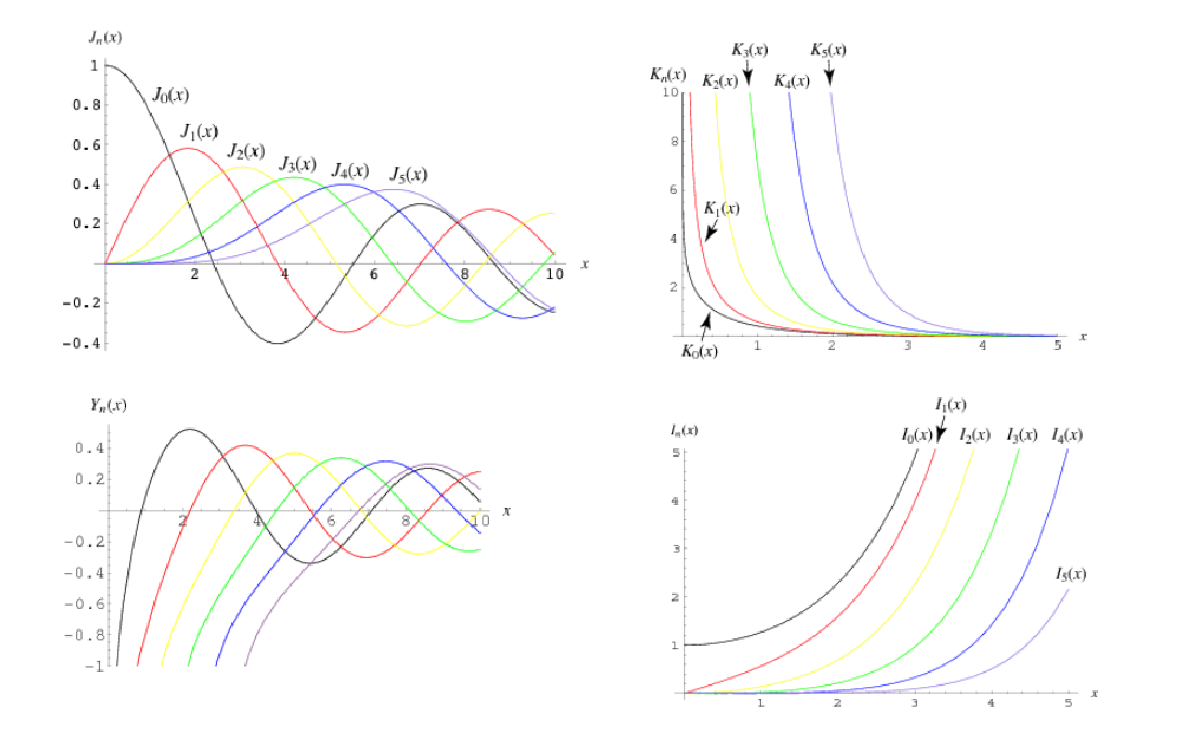
\includegraphics[height = 90mm, width=160mm, angle=0]{bessel.eps}}
\caption{Bessel's functions and modified Bessel's functions, \cite{wolfJ}, \cite{wolfY}. \cite{wolfK}. \cite{wolfI}.}
\label{figure_bessel}
\end{figure}

It is known that the Bessel functions of the first and second kind behave like functions of sine and cosine. Hence, these are candidates for light propagation in the core in the form of a plane wave solution. The logarithmic part of the series solution for $Y_m$ indicates that the solution goes to $-\infty$ as it approaches zero. This could not possibly describe a finite light beam entering the core.  Therefore, the only possible solution in the core is $J_m$ and has real solutions whenever $\beta^2<n_1^2k^2$. Recall that the refractive index in the core and cladding are given by $n_1$ and $n_0$ respectively. Define
\begin{equation}
\begin{array}{c}
E_z=AJ_m(ur)\cos{(m\theta+\alpha)},\\
H_z=BJ_m(ur)\sin{(m\theta+\alpha)},\\
u^2=n_1^2k^2-\beta.
\end{array}
\end{equation}

In the cladding, we require solutions to approach zero as $r\rightarrow\infty$. This is only satisfied by the modified Bessel function of the second kind $K_m(r)$ since the modified Bessel function of the first kind goes to infinity as $r\rightarrow\infty$. For real solutions in the cladding, it is necessary that $\beta^2>n_0^2k^2$.
Define
\begin{equation}
\begin{array}{c}
E_z=CK_m(wr)\cos{(m\theta+\alpha)},\\
H_z=DK_m(wr)\sin{(m\theta+\alpha)},\\
w^2=\beta-n_0^2k^2.
\end{array}\label{cutoff.eqn}
\end{equation}
We may now use these to define the components of the electric and magnetic field in the directions of $r$ and $\theta$ in equations (\ref{TE5.eqn})-(\ref{TE8.eqn}). It follows that
\begin{align*}
E_\theta^{(core)}&=\frac{-i}{u^2}\left((Am\frac{\beta}{r}J_m(ur)+B\omega\mu_0\frac{\partial J_m(ur)}{\partial r}\right)\sin{(m\theta+\alpha)},\\
E_\theta^{(cladding)}&=\frac{-i}{w^2}\left(Cm\beta\frac{\partial K_m(wr)}{\partial r}+D\frac{\omega\mu_0}{r}\frac{\partial K_m(wr)}{\partial\theta}\right)\sin{(m\theta+\alpha)},\\
H_\theta^{(core)}&=\frac{-i}{u^2}\left(Am\frac{\beta}{r}J_m(wr)+B\omega\varepsilon_0 n_1^2\frac{\partial K_m(wr)}{\partial r}\right)\cos{(m\theta+\alpha)},\\
H_\theta^{(cladding)}&=\frac{-i}{w^2}\left(Cm\beta J_m(wr)+D\frac{\omega\varepsilon_0 n_0^2}{r}\frac{\partial K_m(wr)}{\partial\theta}\right)\cos{(m\theta+\alpha)}.
\end{align*}

Recall from subsection \ref{lightrays.sec} that light rays are confined in the core. Total internal reflection only occurs if the refractive index of the core and cladding satisfy $n_1>n_0$, respectively, and only depends on the choice of radius, $r=a$, where the core-cladding boundary is. The boundary conditions for each of the components of the electric and magnetic fields given by equations (\ref{BCs.eqn}) are applied to the equations above involving Bessel functions. The system of equations,
\begin{equation*}
\left(\begin{array}{cccc}
\frac{m\beta}{u^2a^2}J_m(ua)&\frac{k\omega\mu_0}{ua}J'_m(ua)&\frac{m\beta}{w^2a}K_m(wa)&-\frac{k\omega\mu_0}{w^2a}K'_m(wa)\\
\frac{kn_1^2}{ua}J'_m(ua)&\frac{\omega\mu_0m}{u^2a^2}J_m(ua)&\frac{k^2n_0^2}{wa}K'_m(wa)&\frac{\omega\mu_0m\beta}{w^2a^2}K_m(wa)\\
J_m(ua)&0&-K_m(wa)&0\\
0&J_m(ua)&0&K_m(wa)
\end{array}\right)
\left(\begin{array}{c}A\\B\\C\\D\end{array}\right)=
\left(\begin{array}{c}0\\0\\0\\0\end{array}\right),
\end{equation*}
is obtained.

The characteristic equations are a result of finding the determinant of the system of equations and equating it to zero. These are the characteristics corresponding to the solution of Maxwell's wave equation described by the Bessel functions. Characteristics follow the path of light rays and are distributed according to the plane wave solution of $m$ propagation modes. The larger the value of $m$, the more dispersed the modes become and more rays of an initial arbitrary beam are considered. 

The characteristic equations also give the propagation constant $\beta$ and amplitudes $E_z,E_r,E_\theta,H_z,H_r,H_\theta$ whenever $n_1$, $n_0$, $a=\mbox{`core radius'}$ and normalized frequency
$$V=\sqrt{(ua)^2+(wa)^2}=\left[a\sqrt{\mu_0\varepsilon_0(n_1^2-n_0^2)}\right]\omega$$ are given. Knowing the propagation constant and amplitudes allows us to analyze the dispersive solutions and group velocity behaviour according to the definitions and discussion in section \ref{dispersion.sec}.

The normalized group velocity can be found and we may check which modes have non-zero group velocity for a fixed value of $m$ and some value of the normalized frequency, $V$, which in turn depends on some value of the frequency, $\omega$. The normalized group velocity is given as the ratio of the speed of light, $c$, with the actual group velocity, $v_g$, by rewriting $\beta$ and $k$ with respect to the normalized frequency, $V$, and applying the product rule;
$$\frac{c}{v_g}=\frac{d\beta}{d k}=\frac{a\sqrt{n_1^2-n_0^2}}{a\sqrt{n_1^2-n_0^2}}\frac{d(\frac{V\beta}{k})}{dV}=V\frac{d\left(\frac{\beta}{k}\right)}{dV}+\frac{\beta}{k}.$$
If a normalized group velocity is zero for a mode $m$, then there is no dispersion occurring with respect to that mode.

The characteristic equations from the determinant are given as
\begin{multline}
\left(\frac{J'_m(ua)}{uaJ_m(ua)}+\frac{K'_m(wa)}{waK_m(wa)}\right)\left(\frac{J'_m(ua)}{\kappa J_m(ua)}+\frac{n_0^2K'_m(wa)}{n_1^2wa K_m(wa)}\right)\\=m^2\left(\frac{1}{(ua)^2}+\frac{1}{(wa)^2}\right) \left(\frac{n_1^2}{n_0^2}\frac{1}{(ua)^2}+\frac{1}{(wa)^2}\right).\label{characteristic_equation.eqn}
\end{multline}
In general this eigenvalue problem may have several solutions for each integer value of $m$. It is customary to express these solutions by $\beta_{mn}$ where both $m$ and $n$ are integers. An eigenvalue, $\beta{mn}$, corresponds to a mode which the fiber can support. Since we may solve the wave equation for either $\vec{E}$ or $\vec{H}$ then these are designated $HE_{mn}$ and $EH_{mn}$, representing solving the wave equation with respect to $\vec{H}$ and $\vec{E}$ respectively.

Now we consider the most fundamental solutions to the characteristic equations. Let $m=0$, then the characteristic equation, (\ref{characteristic_equation.eqn}), becomes 
\begin{equation}
\left(\frac{J'_m(ua)}{uaJ_m(ua)}+\frac{K'_m(wa)}{waK_m(wa)}\right)\left(\frac{J'_m(ua)}{\kappa J_m(ua)}+\frac{n_0^2K'_m(wa)}{n_1^2wa K_m(wa)}\right)=0\nonumber.
\end{equation}
Then, necessarily
\begin{equation}\left(\frac{J'_m(ua)}{uaJ_m(ua)}+\frac{K'_m(wa)}{waK_m(wa)}\right)=0
\label{TE.eqn}\end{equation}
and
\begin{equation}
\left(\frac{J'_m(ua)}{\kappa J_m(ua)}+\frac{n_0^2K'_m(wa)}{n_1^2wa K_m(wa)}\right)=0.
\label{TM.eqn}
\end{equation}

Equations (\ref{TE.eqn}) and (\ref{TM.eqn}) are the characteristic equations for the TE and TM modes, respectively. Both of these cannot be simultaneously zero unless describing the trivial solution. Notice that whenever (\ref{TE.eqn}) is satisfied, then $A=C=0$ in the system of equations given by the boundary conditions. If $A=C=0$ then $E_z=0$ and we conclude that the electric field does not propagate in the $z$ direction. A similar argument holds for the TM mode using equation \ref{TM.eqn}.

For a given frequency, $\omega$, the normalized group velocities corresponding to values of $\beta$ are obtained from characteristic equations for integer values of $m$. When comparing these group velocities for different values of $\omega$, it is known according to \cite{Belanger}, \cite{Okamoto} and \cite{Agrawal} that the group velocity is zero for all other modes except the TE mode whenever $V_0<2.4$, where the number 2.4 is rounded down from its further approximated decimal expansion. Hence, the TE mode is the only mode that disperses for the corresponding frequency, $\omega_0$, determined by radius $a$ and refractive indices $n_1$ and $n_0$. 
\section{Conclusions}\label{conclusion.sec}
To conclude this report, a summary of what has been discussed is taken up first. Then, ways in which solutions can be further interpreted are discussed. Lastly we state how to begin analyzing non-linear effects in optical fibers.

The goal of this report was to describe light propagation in optical fibers. In order to do this, a description of optical fibers was discussed so that a simple optical fiber could be defined. Doing so also made it possible to interpret the boundary conditions that are involved in a given problem concerning light propagation.

After defining the fixed physical properties of an optical fiber, the general properties of light within glass were discussed. A parametrization of light in the form of rays is given and already simplifies the problem. It was also observed that light takes the form of electromagnetic energy. The equations governing the dynamic properties of electric and magnetic fields were required to describe the light propagating in the core of the fiber. 

Maxwell's equations were used to derive Maxwell's wave equation.  This is the wave equation which governs any electromagnetic waves in an optical fiber and includes the governing of light propagation. Once the necessary equations and boundary conditions have been established, a method of finding solutions was required.

Hyperbolic partial differential equations were introduced and are necessary for defining dispersion in a linear medium. The method of characteristics was used to illustrate an example of a hyperbolic wave. This demonstrated the ray tracing technique that is used when finding solutions to Maxwell's wave equation for optical fibers. This lead to the definition of dispersion, which arose in the plane wave solutions to the initial boundary value problem for the $1$-dimensional wave equation.

By defining dispersion, it became necessary to define group velocity. The group velocity is responsible for the broadening of light and is what causes dispersion to take place only if the phase velocity differs from the group velocity. By deriving the group velocity, we could interpret possible solutions more carefully.

The assumptions, definitions and derivations from sections 1 to 5 were gathered to come up with a solution. The assumption of monochromatic plane wave solutions was made. It also needed to be assumed that only short distances could be considered since the wave equations are non-linear in general. A linear approximation assumption that only describes effects over short distances and small duration in time was made. It was shown that it is possible to use Bessel functions and modified Bessel functions to compute characteristic equations. These equations describe the distribution of propagation modes.

The modal distribution is further interpreted by analyzing the group velocity behaviour. This is done by comparing the normalized frequency $V$ with the normalized propagation constant $\beta\slash k$. The graph of these two related quantities have zeros corresponding to the zeros of the Bessel function $J_m$ and modified Bessel function $K_m$.

The frequencies where these zeros occur correspond to frequencies where modes are `cut off'. For a particular mode $m_0$ to propagate in the core, it must have a sufficiently large normalized frequency, $V_0=\sqrt{(wa)^2+ (ua)^2}$, such that $V_0>2.4$. A larger frequency implies that more modes are being dispersed in the fiber since the corresponding group velocities are non-zero. Therefore, the dispersion increases with increasing frequency, since more modes exist and travel at differing group velocities.

The group velocity behaviour can then be analyzed when the refractive indices are independent of frequency. This depends on the linearization assumption that precluded the definition of light rays and linear dispersive solutions. Non-linear effects may also emerge for a sufficiently large amplitude and short durations of time over long distances. Therefore, sufficiently small amplitudes of light waves entering the core must also be assumed for the linearization assumption to be valid.

Recall that light had been parametrized linearly using the assumption of a local solution in section 2. This was equivalent to the assumption of a linearly approximated index of refraction in glass that does not depend on the frequency.

The refractive index of glass appears in Maxwell's wave equation and, in general, depends on frequency when considering non-linear effects, but this report was only concerned with the linear approximation of Maxwell's wave equation.

The non-linear theory of optical fibers is required to find solutions occurring over long distances, long durations of time and for larger amplitudes. Non-linearity is a consequence of the properties embedded in the material, namely, glass. The assumption of linearity was made in this report by linearly approximating the electric susceptibility, $\chi(E)$, in the corresponding Taylor expansion representing $\chi(E)$. 

In general, the non-linear effects grow over long distances or over long durations of time or for large amplitudes. Using the linear approximation of permittivity allowed us to linearize the problem and solutions obtained in this report are only valid for short distances and short durations of time and small amplitudes.
\appendix
\section{Appendix: Vector Calculus Results}\label{A.sec}
\subsection{The Gradient}
\begin{definition} The \textbf{gradient} is a vector valued differential operator which generalizes the derivative for multivariate functions. It is defined by,
\begin{equation}
\vec{\nabla}\equiv\vec{i}\frac{\partial}{\partial x}+\vec{j}\frac{\partial}{\partial y}+\vec{k}\frac{\partial}{\partial z}
\label{grad.eqn}
\end{equation}
and has the property that
\begin{equation}
du=\vec{\nabla}u\circ d\vec{r}
\label{gradient2.eqn}
\end{equation} 
for an arbitrary function $u(\vec{r})$.
\end{definition}
\subsection{Divergence of a Field}
\begin{definition}The \textbf{divergence} of a field $\vec{A}$ is defined by the projection of the field onto the gradient for each infinitesimal point in space. This is equivalent to the dot product of the gradient with $\vec{A}$ given by,
\begin{equation}
div(\vec{A})=\vec{\nabla}\circ\vec{A}=\lim_{\Delta V\to 0}\frac{1}{\Delta V}\oint_{S}\vec{A}\circ\hat{n}\,da
\label{diver.eqn}
\end{equation}
\end{definition}
\subsection{Divergence Theorem}
\begin{theorem}The flux of a vector field through a closed surface $S$ is equal to the integral of the divergence of the field over a volume $V$ for which $S$ is a boundary. This may be written for some field, $\vec{A}$, as
\label{divthm}
\begin{equation}
\oint_{S}\vec{A}\circ\hat{n}\,da = \int_{V}(\vec{\nabla}\circ\vec{A})\,dV
\label{divthm.eqn}
\end{equation}
\end{theorem}
\subsection{Curl and Circulation of a Vector Field}
The curl and the circulation of a vector field is defined so that Stokes' theorem may be interpreted.
\begin{definition}The \textbf{curl} of a vector field $\vec{A}$ is a \enquote{measure of the vector field's tendency to circulate about a point}(p.75)\cite{Flei}. It is defined,
\begin{equation}
curl(\vec{A})=\vec{\nabla}\times\vec{A}=\lim_{\Delta S\to 0}\frac{1}{\Delta S}\oint_{C}\vec{A}\circ\,d\vec{l}
\label{curl.eqn}
\end{equation}
\end{definition}
\begin{definition}The \textbf{circulation} of a vector field $\vec{A}$ is the magnitude of cumulative force of the vector field along the direction and length of a closed path $C$. Formally this is may be written as,
\begin{equation}
Circulation(\vec{A})=\oint_{C}\vec{A}\circ d\vec{l}
\label{circulation.eqn}
\end{equation}
\end{definition}
\subsection{Stoke's Theorem}
\begin{theorem}The circulation of a vector field over a closed path $C$ is equal to the integral of the normal component of the curl of that field over a surface $S$ for which $C$ is boundary. This may be expressed by the equation,
\begin{equation}
\oint_{C}\vec{A}\circ\,d\vec{l}=\int_{S}(\vec{\nabla}\times\vec{A})\circ\hat{n}\,da
\label{stokes.eqn}
\end{equation}
\end{theorem}
\begin{remark} 
The proofs for the Divergence and Stokes' theorems and the derivations for the gradient, divergence, and curl can be found in \cite{Reitz}.
\end{remark}
\section{Appendix: Differential Equations}
\subsection{Solutions to ODEs Around A Regular Singular Point}\label{ODEintro.sec}
This section of the appendix follows \cite{Codd} to find solutions to Bessel's equation. Bessel's equation is an ODE that is defined in subsection \ref{bessel.sec} First, theorems and definitions for existence and uniqueness of solutions to ODEs around regular singular points are stated. The proof of the theorems can be found in \cite{Codd}.

The method of Frobenius is applied to Bessel's equation in subsection \ref{bessel.sec}. The method of Frobenius is a method of obtaining solutions by supposing a particular series solution exists. The supposed series is inputted into the ODE to obtain a recurrence relation for coefficients in the solution. We seek convergent series solutions by applying the method of Frobenius. The details of this method can be found in \cite{Codd}.
\begin{theorem}\textbf{(Existence of Series Solutions for Analytic Coefficients)}
Let $x_0\in\mathbb{R}$ and suppose the coefficients $a_1,...,a_n$ in
\begin{equation}
L(y)=y^{(n)}+a_1(x)y^{(n-1)}+\cdots+a_n(x)y
\label{b2.eqn}
\end{equation}
have convergent power series expansions in powers of $(x-x_0)$ on an interval $\vert x-x_0\vert<0$ for $r_0>0$. If $\gamma_1,...,\gamma_n$ are any $n$ constants, there exists a solution $\phi$ of the problem $$L(y)=0,\,\,y(x_0)=\gamma_1,\,\,...,\,\,y^{(n-1)}(x_0)=\gamma_n,$$ with a power series expansion
\begin{equation}
\phi(x)=\sum_{k=0}^\infty c_k(x-x_0)^k
\label{b3.eqn}
\end{equation}
convergent for $\vert x-x_0\vert<r_0$. We have
$$c_kk!=\gamma_k+1,\qquad (k=0,1,...,n-1),$$ and $c_k$ for $k\geq n$ may be computed in terms of $c_0,c_1,...,c_{n-1}$ by substituting (\ref{b3.eqn}) into $L(y)=0$.
\end{theorem}
\begin{theorem}\label{thm3}\textbf{(Uniqueness of Solutions)}
Let $x_0\in I\subset\mathbb{R}$, and let $\gamma_1,...,\gamma_n$ be any n constants. There is at most n solutions $\phi$ of $L(y)=0$ on $I$ satisfying
$$ \phi(x_0)=\gamma_1,\,\,\phi'(x_0)=\gamma_2,\,\,...,\,\,\phi^{(n-1)}(x_0)=\gamma_n,$$
where $L(y)$ is the linear differential operator for some ODE applied to the solution.
\end{theorem}
\begin{definition}\textbf{(Regular Singular Point)}
Let $x_0\in\mathbb{R}$ and consider the linear differential equation with variable coefficients
\begin{equation}
a_0(x)y^{(n)}+a_1(x)y^{(n-1)}+\cdots +a_n(x)y=0.
\label{b4.eqn}
\end{equation}
Then $x_0$ is a regular singular point for (\ref{b4.eqn}) if the equation can be written in the form
$$(x-x_0)^ny^{(n)}+b_1(x)(x-x_0)^{(n-1)}y^{(n-1)}+\cdots+b_n(x)y=0$$ near $x_0$, where the functions $b_1,...,b_n$ are analytic at $x_0$. 
\end{definition}
\begin{theorem}\label{thm1}\textbf{(Series Solutions Near a Regular Singular Point)}
Consider the equation
$$x^2y''+a(x)xy'+b(x)y=0$$
where $a,b$ have convergent power expansions for $\vert x\vert<r_0$ and $r_0>0$. Let $r_1,r_2$ satisfy $Re(r_1)\geq Re(r_2)$ and be the roots of the indicial polynomial
$$q(r)=r(r-1)+a(0)r+b(0).$$
For $0<\vert{x}\vert<r_0$ there is a solution $\phi_1$ of the form
$$\phi_1(x)=\vert{x}\vert^{r_1}\sum_{k=1}^\infty c_kx^k,\quad (c_0=1),$$
where the series converges for $\vert{x}\vert<r_0$. If $(r_1-r_2)\neq 0$ or $(r_1-r_2)=N\in\mathbb{Z}^{+}$, there is a second solution $\phi_2(x)$ for $0<\vert{x}\vert<r_0$ of the form
$$\phi_2(x)=\vert{x}\vert_{r_2}\sum_{k=0}^\infty \tilde{c}_kx^k,\quad(\tilde{c}_0=1),$$
where the series converges for $\vert{x}\vert<r_0$. The coefficients $c_k$ and $\tilde{c}_k$ can be obtained by substitution of the solutions into the differential equation.
\end{theorem}
\begin{remark}
The \textbf{method of Frobenuis} refers to the method of obtaining the indicial polynomial by substituting the series solution into the given differential equation. The Frobenius method is used to find values of $r$ for which the series solution proposed in the theorem satisfies the differential equation being considered.
\end{remark}

The second solution in the theorem above is known to exist for $r_1\neq r_2$ by the existence and uniqueness theorems and the fact that $\phi_1,\phi_2$ are linearly independent for non-trivial solutions. There are two exceptional cases for determining the second solution in the theorem above. First, if $(r_1-r_2)=0$ then the solutions $\phi_1$ and $\phi_2$ are no longer linearly independent and another solution is constructed using the method in section 4.6 of \cite{Codd}.

The author of \cite{Codd} also derives a second solution for a second exceptional case, that is, $(r_1-r_2)=N\in\mathbb{Z}^{+}$. Defining the coefficients of the second series solution, in this case, may result in a denominator of zero for a coefficient $\tilde{c}_k$, for some integer $k\geq 1$. Hence, another linearly independent series solution is constructed such that coefficients cannot have zero in the denominator. The next theorem summarizes the results of these special cases.
\begin{theorem}\label{thm2}\textbf{(Special Cases for Solutions Near a Regular Singular Point)}
Consider the same assumptions as theorem \ref{thm1}, except that $(r_1-r_2)$ satisfies either $(r_1-r_2)=0$ or $(r_1-r_2)=N\in\mathbb{Z}^{+}$. In the first case, there are two linearly independent solutions $\phi_1,\phi_2$ for $0<\vert{x}\vert<r_0$ of the form
$$\phi_1(x)=\vert{x}\vert^{r_1}\sigma_1(x),\quad\phi_2(x)=\vert{x}\vert^{r_1}\sigma_2(x)+(log|x|)\phi_1(x),$$
where $\sigma_1,\sigma_2$ have power series expansions which are convergent for $|x|<r_0$, and $\sigma_1(0)\neq 0$. In the second case, there are two linearly independent solutions $\phi_1,\phi_2$ for $0<|x|<r_0$ of the form
$$\phi_1(x)=|x|^{r_1}\sigma_1(x),\quad \phi_2(x)=|x|^{r_2}\sigma_3(x)+A\phi_1(x)log|x|,$$
where $\sigma_1,\sigma_2,\sigma_3$ have power series expansions which are convergent for $|x|<r_0$, $\sigma_1(0)\neq 0$, $\sigma_2(0)\neq 0$, and $c$ is a constant that may be zero.
\end{theorem}
\subsection{Bessel's Equation}\label{bessel.sec}
Bessel's equation of order $\alpha$ is a second order linear ordinary differential equation. Let $\alpha\,\epsilon\,\mathbb{C}$ be a constant such that $Re(\alpha)\geq 0$. Bessel's equation of order $\alpha$ is given as
\begin{equation}
\frac{d^2y}{dx^2}+\frac{1}{x}\frac{dy}{dx}+\bigg(1-\alpha^2\bigg)y=0
\label{b1.eqn}
\end{equation}

The theorems from subsection \ref{ODEintro.sec} are now applied to Bessel's equation of order $\alpha$ to find possible solutions using the method of Frobenius, which is defined in \cite{Codd}. The method of Frobenius is a general method used to prove theorem \ref{thm1} and is not discussed here in full detail. It will, however, be referred to for some justification in applying theorems \ref{thm1} and \ref{thm2} as needed. 

Recall Bessel's equation, (\ref{b1.eqn}), and apply the definition of a regular singular point by writing the equation as
$$x^2y''+xb_1(x)y'+b_2(x)y=0,$$
where $b_1(x)=1$ and $b_2(x)=(x^2-\alpha^2)$ are analytic at $x=0$. Theorem \ref{thm1} is applied to find the first solution for integer values of $\alpha$. This gives the indicial equation satisfying
$$q(r)=r(r-1)+b_1(0)r+b_2(0)=r^2-\alpha^2=(r_1-\alpha)(r_2+\alpha)=0.$$
It follows that $r=\pm\alpha$. The indicial equation is obtained, in general, by inputting a solution of the form
$$\sum_{k=0}^\infty c_kx^{k+r}$$ into the differential equation. Doing so follows from the method of Frobenius. Inputting this solution into Bessel's equation gives,
\begin{align}
0&=x^2\sum_{k=0}^\infty c_k(k+r)(k+r-1)x^{k+r-2}+x\sum_{k=0}^\infty c_k(k+r)x^{k+r-1}+(x^2-\alpha^2)\sum_{k=0}^\infty c_kx^{k+r}\nonumber\\
&=\sum_{k=0}^\infty c_k\Big((k+r)(k+r-1)+(k+r)-\alpha^2\Big)x^{k+r}+\sum_{k=0}^\infty c_{k-2}x^{k+r}\nonumber\\
&=q(r)c_0x^r+q(r+1)c_1x^{r+1}+\sum_{k=2}^\infty\Big(q(r+k)c_k+c_{k-2}\Big)x^{k+r}.
\label{indicialform.eqn}
\end{align}
When $k=k_0$ we recover the terms proportional to $x^{r+k_0}$. It follows by the method of Frobenius that $k=0$ gives
$$0=q(r)c_0x^r.$$
The method also implies $c_0\neq 0$, since otherwise $c_k=0,\quad\forall\,k\geq 0$, and gives a trivial solution in defining a recurrence relation. Also, $x^r\neq 0$, since $x>0$. Therefore, the indicial polynomial, $q(r)$, is necessarily zero to obtain non-trivial solutions. It is also necessary that $c_1=0$ by linear independence with respect to powers of $x$, and since $x^{r+1}\neq 0$ and inputting $r=\pm\alpha$ gives
$$q(r+1)=(1\pm\alpha+\alpha)(1\pm\alpha-\alpha)=\left\{ \begin{array}{rcl}
1+2\alpha & \mbox{for}&r=\alpha\\
1-2\alpha & \mbox{for}&r=-\alpha
\end{array}\right.\neq 0,\quad\forall\,\alpha\in\mathbb{R}.$$
It follows from (\ref{indicialform.eqn}) that coefficients of the infinite series are necessarily zero. Then, a recurrence relation may be defined as
\begin{equation}
C_k(r)=\frac{-c_{k-2}}{(k+r-\alpha)(k+r+\alpha)}.
\label{ck.eqn}
\end{equation}
The recurrence relation gives coefficients of every other integer value subscript. Now, let $r=r_1=\alpha$ to obtain the even and odd coefficients, computed from $c_0$ and $c_1$, respectively, of the series solution with $r=\alpha$. It follows that
$$C_k(0)=c_k=\frac{-c_{k-2}}{k(2\alpha+k)},$$
by inputting $r=\alpha$. This relation is used to compute even coefficients $c_{2m}$ for integers $m>0$. All odd coefficients are zero because $c_1=0$. By computing the first few values of the recurrence relation,
\begin{equation}
c_{2m}=\frac{(-1)^mc_0}{m!2^{2m}(\alpha+m)\cdot...\cdot(\alpha+1)},
\label{rec1.eqn}
\end{equation}
is obtained. Consider $\alpha\in\{0,1,2,3,...\}$ and recall that $c_0$ is a constant that can be chosen arbitrarily. If $\alpha=0$ we can choose $c_0=1$ so that (\ref{rec1.eqn}) can be written as
$$c_{2m}=\frac{(-1)^mc_o}{2^{2m}(m!)^2}.$$
Therefore, by theorem \ref{thm1}, the solution to Bessel's equation of order $\alpha=0$ is
\begin{equation}
J_0(x)=\sum_{m=0}^\infty\frac{(-1)^mx^{2m}}{2^{2m}(m!)^2}
\label{bessel0.eqn}
\end{equation}
For integers $\alpha=n\geq 1$, we may choose $C_0(n)=1\slash(2^nn!)$ to obtain
\begin{equation}
C_{2m}(n)=\frac{(-1)^m}{2^{2m+n}m!(m+n)!}.
\label{nc2m.eqn}
\end{equation}
These coefficients give solutions to Bessel's equation of order $\alpha=n$, for integers $n>0$. The choice of $C_0(n)$ guarantees the series converges. Such solutions are given by
\begin{equation}
J_n(x)=\sum_{m=0}^\infty\frac{(-1)^mx^{2m+n}}{2^{2m+n}m!(m+n)!}.
\label{besseln.eqn}
\end{equation}

Next, we introduce the gamma function and its properties. We use it to define a particular $C_0(\alpha)$. The motivation of defining $C_0(\alpha)$ using the gamma function, is to find a series solution to Bessel's equation of order $\alpha$ for any non-negative value of $\alpha$ such that the solution converges.
\begin{definition}\textbf{(Gamma Function)}
Let $z\in\mathbb{C}$ satisfy $Re(z)\geq 0$. The gamma function is defined by the integral
$$\Gamma(z)=\int_0^\infty x^{z-1}e^{-x}dx.$$ The gamma function satisfies the following properties:
\begin{enumerate}
\item$\Gamma(z+1)=z\Gamma(z)$.
\item$\Gamma(1)=1$.
\item$\Gamma(n)=n\Gamma(n-1)=...=(n-1)!\Gamma(1)=(n-1)!$.
\end{enumerate}
\end{definition}
Observe that choosing
$$C_0(\alpha)=\frac{1}{2^\alpha\Gamma(\alpha+1)}$$
implies that the recurrence can be written
\begin{equation}
C_{2m}(\alpha)=\frac{(-1)^m\alpha!}{2^{2m+\alpha}m!(m+\alpha)!\Gamma(\alpha+1)}=\frac{(-1)^m}{2^{2m+\alpha}m!\Gamma(m+\alpha+1)},
\label{ac2m.eqn}
\end{equation}
which gives a convergent series solution to Bessel's equation of arbitrary order $\alpha$, called a Bessel function, given by
\begin{equation}
J_\alpha(x)=\sum_{m=0}^\infty\frac{(-1)^mx^{2m+\alpha}}{2^{2m+\alpha}m!\Gamma(m+\alpha+1)}.
\label{bessela.eqn}
\end{equation}

Now that we have defined the first solution to Bessel's equation of order $\alpha$, we must find a second linearly independent solution. Whenever $(r_1-r_2)\neq 0$ and $(r_1-r_2)\neq N\in\mathbb{Z}^{+}$ we may apply theorem \ref{thm1} directly and obtain the second linearly independent solution, $J_{-\alpha}(x)$. This may be done by following the proof of convergence for the series solution found on page 160-162 of \cite{codd}, but the details will not be pursued here. $J_\alpha(x)$ and $J_{-\alpha}(x)$ are two necessarily different solutions. Hence, whenever $r_1-r_2\neq 0$, then $J_\alpha(x)$ and $J_{-\alpha}(x)$ are the two linearly independent solutions corresponding to the series with coefficients $C_k(r_1)$ and $C_k(r_2)$, respectively.

Consider either of the special cases $(r_1-r_2)=0$ or $(r_1-r_2)=N\in\mathbb{Z}^{+}$. Theorem \ref{thm2} is applied to each case, following the method of Frobenius, to get the second solution as required. Recall theorem \ref{thm2}. The arguments involved in finding a second solution for these special cases, that are indeed linearly independent from the first, is not discussed here. Those details are given in \cite{Codd}. Define $(r-r_2)C_k(r)=\tilde{C}_k(r)$. In summarizing the arguments mentioned above, we obtain
\begin{align}
&\sigma_1(x)=\sum_{k=0}^\infty C_k(r_1)x^k,\qquad\sigma_2(x)=\sum_{k=0}^\infty x^k\bigg[\frac{d}{dr}C_k(r)\bigg]\bigg|_{r=r_1},\label{secondsol1.eqn}\\
&\sigma_3(x)=\sum_{k=0}^\infty x^k\bigg[\frac{d}{dr}(r-r_2)C_k(r)\bigg]\bigg|_{r=r_2},\qquad A=(r-r_2)C_N(r)\big|_{r=r_2}.\label{secondsol2.eqn}
\end{align}
Now, we can find another pair of solutions to Bessel's equation of order $\alpha$ using these equations; by solving for the coefficients
$$C_k(r_1),\quad\frac{d}{dr}C_k(r_1),\quad\frac{d}{dr}\tilde{C}_k(r_2)=\bigg[\frac{d}{dr}(r-r_2)C_k(r)\bigg]\bigg|_{r=r_2},\quad A= \tilde{C_N}(r_2),$$
according to theorem \ref{thm2}.

In order to take these derivatives, we must obtain an equation for $C_k(r)$, given by (\ref{ck.eqn}), with respect to only $r$ and $k$. We can find $C_k(r)$ as required by computing the first few terms. It follows that
\begin{align*}
C_0(r)&=C_0,\qquad (\text{for some constant }C_0),\\
C_2(r)&=\frac{-C_0}{(r+2+\alpha)(r+2-\alpha)},\\
C_4(r)&=\frac{-C_2(r)}{(r+4+\alpha)(r+4-\alpha)}=\frac{C_0}{(r+2+\alpha)(r+2-\alpha)(r+4+\alpha)(r+4-\alpha)},\\
C_6(r)&=\frac{-C_4(r)}{(r+6+\alpha)(r+6-\alpha)}=\frac{-C_0}{\prod_{k=1}^3(r+2k+\alpha)(r+2k-\alpha)}, ...,
\end{align*}
which gives
\begin{equation}
C_{2m}(r)=\frac{C_0(-1)^m}{\prod_{k=1}^m(r+2k+\alpha)(r+2k-\alpha)}.
\label{c2m.eqn}
\end{equation}
In order to apply the product rule in differentiating $\tilde{C}_{2m}(r)$, we require
$$C_{2m}(r)'=[C_0(-1)^md_{2m}(r)]',$$
where
$$d_{2m}(r)=\frac{1}{\prod_{k=1}^m(r+2k+\alpha)(r+2k-\alpha)}.$$
Observe that
$$\frac{d}{dr}\log{d_{2m}(r)}=\frac{\frac{d}{dr}d_{2m}(r)}{d_{2m}(r)},$$
by applying the chain rule. It follows that
$$\frac{d}{dr}\log{d_{2m}(r)}=\Big(-\sum_{k=1}^m\frac{d}{dr}(r+2k+\alpha)(r+2k-\alpha)\Big)=-2\sum_{k=1}^m(r+2k).$$
Therefore,
\begin{equation}
C'_{2m}(r)=\Bigg[\frac{-2C_0(-1)^m\sum_{k=1}^m(r+2k)}{\prod_{k=1}^m(r+2k+\alpha)(r+2k-\alpha)}\Bigg].
\label{c2m'.eqn}
\end{equation}
Moreover, we may now differentiate $\tilde{C}_{2m}(r)$ using this equation and the product rule. It follows that
\begin{equation}
\frac{d}{dr}\tilde{C}_{2m}(r)=(r-r_2)C'_{2m}(r)+C_{2m}(r).
\label{tildec2m'.eqn}
\end{equation}

The dependence on $\alpha$ is removed in (\ref{c2m'.eqn}) above for the special case of $(r_1-r_2)=0$ from theorem \ref{thm2}, since we have a condition $(r_1-r_2)=2\alpha$. For the case where $(r_1-r_2)=0=2\alpha$, we obtain $\alpha=0$. Then according to theorem \ref{thm2} and equations (\ref{c2m.eqn}), (\ref{c2m'.eqn}) and (\ref{bessel0.eqn}) we obtain the first solution, $J_0(x)$, and the second linearly independent solution,
$$B(x)=J_0(x)\log{|x|}+\sum_{m=0}^\infty\Bigg(\frac{-2C_0(-1)^m\sum_{k=1}^m(r+2k)}{\prod_{k=1}^m(r+2k)^2}\Bigg)x^{2m}.$$
Then, according to theorem \ref{thm3}, the solution to Bessel's equation of order zero is
\begin{equation}
c_2J_0(x)+c_3B(x)
\label{fullbessel0.eqn}
\end{equation}
for constants $c_2,c_3$ satisfying some initial conditions.

Similar to the first case, we obtain a second linearly independent solution for the case $(r_1-r_2)=2\alpha=N\in\mathbb{Z}^{+}$ using theorem \ref{thm2}, except it is for general $\alpha$. Recall that $r_2=-\alpha$. Then by equation (\ref{c2m.eqn}) and the equation $2m=N=2\alpha$, we obtain
\begin{equation}
A=\bigg[(r+\alpha)\frac{C_0(-1)^\alpha}{\prod_{k=1}^\alpha(r+2k+\alpha)(r+2k-\alpha)}\bigg]\bigg|_{r=-\alpha}=\frac{C_0(-1)^{-\alpha}}{(2\alpha)\prod_{k=1}^{\alpha-1}4k(k-\alpha)}.
\label{A.eqn}
\end{equation}
According to theorem \ref{thm2} and equations (\ref{bessela.eqn}), (\ref{c2m'.eqn}), (\ref{tildec2m'.eqn}) and (\ref{A.eqn}) we obtain the first solution, $J_\alpha(x)$, and the second linearly independent solution,
$$|x|^\alpha\sum_{m=0}^\infty\Big((r+\alpha)C_{2m}(r)'+C_{2m}(r)\Big)x^{2m}+\bigg[\frac{C_0(-1)^{-\alpha}}{(2\alpha)\prod_{k=1}^{\alpha-1}4k(k-\alpha)}\bigg]J_\alpha(x)\log{|x|},$$
denoted by $Y_\alpha(x)$. Note that $Y_\alpha(x)$ is called the Bessel function of the second kind. Then, according to theorem \ref{thm3}, Bessel's equation of order $\alpha$ has the solution
\begin{equation}
c_4J_\alpha(x)+c_5Y_\alpha(x),
\label{fullbesselN.eqn}
\end{equation}
whenever $\alpha=N\slash 2\in\mathbb{Z}^{+}$.
\subsection{The Modified Bessel's Equation}\label{modified_bessel.sec}
For applying Bessel's equation in section \ref{guides.sec}, we must consider complex values of $x$ which have no real part in Bessel's equation, (\ref{b1.eqn}). In this case, the Bessel functions \textit{may} not be solutions to Bessel's equation because the way that Bessel's equation is written becomes different. This is relevant for finding solutions according to the theorems in appendix \ref{ODEintro.sec}. It is possible to modify Bessel's equation to be suitable for $ix\in\mathbb{C}$ satisfying $Re(ix)=0$. This subappendix deals with finding real solutions with respect to $x\in\mathbb{R}$ that are also solutions with respect to the variable $ix\in\mathbb{C}$ for a modified version of Bessel's equation.

The transformation $x\mapsto ix$ is applied to Bessel's equation and gives an equation called the modified Bessel's equation. The same method of finding solutions as for Bessel's equation is used to find real series solutions centered at $x=0,\quad x\in\mathbb{R}$ corresponding to the imaginary variable $ix$.

The modified Bessel's equation is given by
$$(ix)^2y''+ixy'+\big((ix)^2+\alpha^2\big)y=0.$$
Applying the method of Frobenius in the same way as for Bessel's equation gives the required condition for the indicial equation by the relation
\begin{equation}
0=q(r)c_0(ix)^r=(r-\alpha)(r+\alpha)c_0i^rx^r.
\label{bmod1.eqn}
\end{equation}

Following the same argument as for Bessel's equation, we have $i^r\neq 0$ for any value of $r$. Hence, the indicial equations for both regular and modified Bessel's equation are the same and given by $q(r)$ above. The series solution,
\begin{equation}
\sum_{k=0}^\infty C_k(r)(ix)^{r+k},
\label{bmod2.eqn}
\end{equation}
can be written with respect to powers of $x$ by factoring out $i^r$ in (\ref{bmod1.eqn}). Doing so means that the series must be written as
\begin{equation}
\sum_{k=0}^\infty C_k(r)x^r(ix)^k.
\end{equation}

Whenever coefficients are real, the series solution is real only for even values of $k$. This also introduces a factor of $-1$ for each coefficient. It is now shown by substituting the series solution, (\ref{bmod2.eqn}), into the modified Bessel's equation that, indeed, only even values of k occur in the series solution and the coefficients are real. Substituting the series solution gives
\begin{multline}
0=(ix)^2\sum_{k=0}^\infty C_k(r)(k+r)(k+r-1)(ix)^{k+r-2}+ix\sum_{k=0}^\infty C_k(r)(k+r)(ix)^{k+r-1}\\+\big((ix)^2-\alpha^2\big)\sum_{k=0}^\infty C_k(r)(ix)^{k+r}\nonumber
\end{multline}
\begin{align}
&=\sum_{k=0}^\infty C_k(r)\Big((k+r)(k+r-1)+(k+r)-\alpha^2\Big)(ix)^{k+r}-\sum_{k=0}^\infty C_{k-2}(r)(ix)^{k+r}\nonumber\\
&=q(r)C_0(ix)^r+q(r+1)C_1(r)(ix)^{r+1}+\sum_{k=2}^\infty\Big(q(r+k)C_k(r)-C_{k-2}(r)\Big)(ix)^{k+r}.
\label{bmod3.eqn}
\end{align}

By the same arguments as for the Bessel's equation, we have that $c_1=0$. Hence, the recurrence is given only for even values of $k$, since the coefficients of the series satisfy
$$q(r+k)C_k(r)-C_{k-2}(r)=0.$$
The factor of $-1$ must also be introduced in the term,
$$\sum_{k=2}^\infty\Big(q(r+k)C_k(r)-C_{k-2}(r)\Big)(ix)^{k+r},$$
above. In doing so, it may be rewritten as
$$\sum_{k=2}^\infty\Big(C_{k-2}(r)-q(r+k)C_k(r)\Big)(ix)^rx^k,$$
and satisfies
$$0=\sum_{k=2}^\infty\Big(C_{k-2}(r)-q(r+k)C_k(r)\Big)x^{k+r},$$
since $q(r)=0$ and $c_1=0$ in equation (\ref{bmod3.eqn}).

This gives the recurrence relation
\begin{equation}
C_k(r)=\frac{C_{k-2}(r)}{(r+k+\alpha)(r+k-\alpha)}
\label{bmod4.eqn}
\end{equation}
This recurrence relation is like the one from equation (\ref{ck.eqn}) for Bessel's equation, except with a factor of $-1$. Therefore, the procedure for finding first and second linearly independent solutions corresponding to the cases in theorems \ref{thm1} and \ref{thm2} is practically the same for the modified Bessel equation as it is for Bessel's equation. The coefficients of these series solutions for the modified Bessel's equation,
$$C_k^{mod}(r_1),\quad\frac{d}{dr}C_k^{mod}(r_1),\quad\frac{d}{dr}\tilde{C}_k^{mod}(r_2)=\bigg[\frac{d}{dr}(r-r_2)C_k^{mod}(r)\bigg]\bigg|_{r=r_2},\quad A= \tilde{C}_N^{mod}(r_2),$$
can be found by `modifying' the coefficients of the solutions to Bessel's equation according to the transformation
\begin{equation}
\frac{d}{dr}C_{2m}^{mod}(r)=\frac{1}{(-1)^m}\frac{d}{dr}C_{2m}(r),
\label{bmod5.eqn}
\end{equation}
where $C_{2m}(r)$ is defined by (\ref{c2m.eqn}).

First, the two linearly independent solutions in theorem \ref{thm1} are found for the modified Bessel equation, (i.e., for the case $r_1-r_2\neq 0$). Applying the transformation (\ref{bmod5.eqn}) to each coefficient for Bessel's functions obtains the coefficients for the modified Bessel functions. The result of this is given by
$$C_{2m}^{mod}(r)=\frac{C_0(r)}{2^{2m}(m!)^2}.$$

In order to ensure the coefficients provide a convergent series, let 
$$C_0^{mod}(n)=\frac{1}{2^nn!}\qquad\mbox{and}\qquad C_0^{mod}(\alpha)=\frac{1}{2^\alpha\Gamma(1+\alpha)},$$
since these may be chosen arbitrarily. Then the coefficients corresponding to the series solutions of the modified Bessel's equation, according to the assumptions of theorem \ref{thm1}, are given by
\begin{equation}
C_{2m}^{mod}(n)=\frac{1}{2^{2m+n}m!(m+n)!}
\label{bmod6.eqn}
\end{equation}
and
\begin{equation}
C_{2m}^{mod}(\alpha)=\frac{\alpha!}{2^{2m+\alpha}m!(m+\alpha)!\Gamma(1+\alpha)}.
\label{bmod7.eqn}
\end{equation}

Therefore, the modified Bessel's function of the first kind can be defined for either integer values of $\alpha=n$ or arbitrary values of $\alpha$, and is given by
\begin{equation}
I_n(x)=\sum_{m=0}^\infty\frac{(x\slash 2)^{2m+n}}{m!(m+n)!}
\end{equation}
or
\begin{equation}
I_\alpha(x)=\frac{(x\slash 2)^{2m+\alpha}}{m!\Gamma(m+\alpha+1)},
\end{equation}
respectively. The two solutions $I_\alpha(x)$ and $I_{-\alpha}(x)$ form a basis for any other solution of the modified Bessel's equation for the case that $(r_1-r_2)\neq 0$. It remains to find the second linearly independent solutions for the two special cases in theorem \ref{thm2}.

When $r_1-r_2=0$, note that $(r_1-r_2)\slash 2=\alpha=0$ gives the first solution $I_0(x)$. For the second solution we require
$$\frac{d}{dr}C_{2m}^{mod}(r).$$
It is obtained by applying (\ref{c2m'.eqn}) to the transformation (\ref{bmod5.eqn}). Doing so obtains
\begin{equation}
\frac{d}{dr}C_{2m}^{mod}(-\alpha)=\frac{-2m(m+1)}{\prod_{k=1}^m(2k)^2}=\frac{-1}{2^{2m-1}}\bigg[\frac{1}{(m-1)!}+\frac{1}{m!(m-1)!}\bigg].
\label{bmod8.eqn}
\end{equation}
Therefore, the second series solution is given by
\begin{equation}
M(x)=I_0(x)\log{|x|}+\sum_{m=0}^\infty \frac{-2m(m+1)}{\prod_{k=1}^m 
(2k)^2}x^{2m}
\label{bmod9.eqn}
\end{equation}

Now, consider the case $r_1-r_2=N\in\mathbb{Z}^{+}$. The coefficients
$$\bigg[\frac{d}{dr}(r-r_2)C_k^{mod}(r)\bigg]\bigg|_{r=r_2},\quad A= \tilde{C}_N^{mod}(r_2),$$
are given by the transformation, (\ref{bmod5.eqn}), and equations (\ref{tildec2m'.eqn}) and (\ref{A.eqn}). By assumption, $N=2\alpha=2m_0$ for some integer $m_0>0$. It follows that the second solution, called the MBF of the second kind, is given by
\begin{equation}
K_\alpha(x)=\frac{C_0I_\alpha(x)\log{|x|}}{2\alpha 4^{\alpha-1}(\alpha-1)!\prod_{k=1}^{\alpha-1}(k-\alpha)}+|x|^{-\alpha}\sum_{m=0}^\infty\frac{C_0\Big(1-4\alpha\big(\frac{2k(2k+1)}{2}-m\alpha\big)\Big)}{4^mm!\prod_{k=1}^m(k-\alpha)}.
\end{equation}

Note that this does converge by inspecting the coefficients in the series. Therefore, the full solution to the modified Bessel's equation for the case $r_1-r_2=N\in\mathbb{Z}^{+}$ is given by
$$\phi_2(x)=c_6K_\alpha(x)+c_7I_\alpha(x),$$
for some constants $c_6,c_7$.
\subsection{Defining PDEs and Initial Boundary Value Problems}
\label{DEs}
In this section, definitions, theorems and other statements involving differential equations are provided. These statements mainly come from course notes and the preliminary chapters in \cite{Codd}.
\begin{definition}\textbf{(Partial Derivative)}
If $u:\mathbb{R}^n\rightarrow\mathbb{R}$ is a function of $n$ variables $x_1,...,x_n$, then the partial derivative of $u$ with respect to some variable $x_i,\quad i=1,...,n$ at some point $\vec{x}_0=(x_{(1,0)},x_{(2,0)},...,x_{(n,0)})\in\mathbb{R}^2$ is defined as 
$$u_{x_i}(\vec{x}_0)=\frac{\partial u}{\partial x_i}=\lim_{h\rightarrow 0}\frac{u(x_{(1,0)},...,x_{(i,0)}+h,...,x_{(n,0)})-u(x_{(1,0)},...,x_{(n,0)})}{h}.$$
For higher derivatives this may be generalized. For example,
$$u_{x_ix_j}(\vec{x}_0)=\frac{\partial^2u}{\partial x_i\partial x_j}=\lim_{h\rightarrow\infty}\frac{u(x_{(1,0)},...,x_{(i,0)}+h,...,x_{(j,0)}+h,...,x_{(n,0)})-u(x_{(1,0)},...,x_{(n,0)})}{h}.$$
\end{definition}
\begin{definition}\textbf{(Partial Differntial Equation)}
A partial differential equation (PDE) for a function $u$ of the independent variables $x_1,...,x_n$ is an equation of the form
$$F(x_1,...,x_n,...,u,u_{x_1},...,u_{x_n},u_{x_1x_2},...,u_{x_1x_n},...),$$
where $F$ is a given function of the independent variables $x_1,...,x_n$ of the unknown function $u$ and of its partial derivations. The {\it order} of a PDE is the order of the highest partial derivative that appears in $F$.
\end{definition}
\begin{definition}\textbf{(System of PDEs)}
A system of PDEs is defined by one or more unknown functions each corresponding to its own PDE. The order of a system of PDEs is the order of the highest derivative that appears in any of the individual PDEs.
\end{definition}

We restrict statements about PDEs from this point on to those that are no more than second order with four independent variables $x_1,x_2,x_3,x_4$. This makes definitions and theorems directly applicable to the differential equations involved in this report. The following statements may be generalized for higher orders and for more independent variables.

Whenever mixed partial derivatives are equal there is usually simplifications which occur in analyzing PDEs. We state the following theorem to get a general condition that implies the equality of mixed partial derivatives.
\begin{theorem}\textbf{(Clairaut's Theorem)}
If $u$ is defined on the closed ball $B$ that contains the point $\vec{x}_0=(x_{(1,0)},x_{(2,0)},x_{(3,0)},x_{(4,0)}$ and mixed partial derivatives $u_{x_ix_j},u_{x_jx_i}$ are continuous on $B$, then
$$u_{x_ix_j}(\vec{x}_0)=u_{x_jx_i}(\vec{x}_0).$$
\end{theorem}
\begin{definition}\textbf{(Solution to PDE)}
A function $u(x_1,x_2,x_3,x_4)$ is a solution to the PDE,
\begin{equation}
F(x_1,...,x_4,u_{x_1},...,u_{x_4},u_{x_1x_2},...)=0,
\label{DE1.eqn}
\end{equation}
whenever substituting $u$ and its partial derivatives into (\ref{DE1.eqn}), it is satisfied identically in some region $\Omega\subset\mathbb{R}^4$
\end{definition}
\begin{remark}
If the independent variables exist in $\mathbb{R}^4$ for some PDE, then all of the partial derivatives are continuous. This assumption implies that mixed partial derivatives are equal by Clairaut's theorem above.
\end{remark}
\begin{definition}\textbf{(Non-linear, Linear, Semi-Linear and Quasi-Linear PDEs)}
Consider a PDE with unknown function $u(x_1,x_2,x_3,x_4)$. The PDE is linear in its definition without any additional assumptions on dependent or independent variables in $F$. The PDE is linear if it is linear in the unknown function $u$ and its derivatives. The PDE is \it{semi-linear} if it is linear with respect to the highest derivatives, but not necessarily with respect to lower order terms. The PDE is \it{quasi-linear})if it is linear only with respect to its highest derivatives.
\end{definition}
\begin{remark}
Let the sets $N,L,S,Q$ be the set of non-linear, linear, semi-linear, and quasi-linear PDEs, respectively. Then, $N\subset L\subset S\subset Q$.
\end{remark}
\begin{definition}\textbf{(Linear Differential Operator)}
A linear differential operator is a transformation of one function to another. Let $\Omega\subset\mathbb{R}^4$ and $\vec{x}\in\Omega$. A linear differential operator is a linear operator which maps $u(\vec{x})\longmapsto v(\vec{x})$, where the process mapping $u$ to $v$ is partial differentiation. We represent PDEs with linear differential operators. For example,
$$u(\vec{x})\overset{\mathcal{L}}{\longrightarrow}\frac{\partial^2u}{\partial t^2}-\frac{\partial^2u}{\partial x^2}=v(\vec{x}).$$
\end{definition}
In general, we may represent PDEs with linear differential operators. Note that `linear', here, only refers to linearity of the operator. An operator, $\mathcal{O}$, is linear if for some functions, $u,v$, and constant $\gamma$, it satisfies
$$\mathcal{O}[\gamma u+v]=\gamma\mathcal{O}[u]+\mathcal{O}[v].$$

Consider the domain $\Omega\subset\mathbb{R}^4$ with points, $(x,y,z,t)$, representing independent variables of a PDE. Let $u$ be the unknown function for the PDE given by
\begin{equation}
\mathcal{L}[u]=H(x,y,z,t),
\label{L.eqn}
\end{equation}
for some function $H(x,y,z,t)$. This is called a non-homogeneous PDE and it can be shown, in general, that any non-homogeneous PDE can be transformed into a homogeneous PDE with a possibly different unknown function $\bar{u}$ and transformed functionf $f_i(x,y,z,t)\longmapsto g_i(x,y,z,t))$ for some functions $g_i(x,y,z,t)$.
\begin{definition}\textbf{(Initial Bounary Value Problem)}
Let the operator (\ref{L.eqn}) define a PDE. The PDE defines an initial boundary value problem (IBVP). An IBVP for the PDE is given by the system of PDEs,
\begin{align}
\mathcal{L}[u]&=0,\\\nonumber
\mathcal{L}_1[u]&=f_1(x,y,z,t),\\\nonumber&\,...,\\\nonumber \mathcal{L}_k[u]&=f_k(x,y,z,t),
\label{system.eqn}
\end{align}
where $\mathcal{L}_i$ are other linear differential operators, also having unknown function $u$.
\end{definition}
\begin{definition}\textbf{(Well-Posed IBVP)}
An IBVP is well-posed if it satisfies the following:
\begin{enumerate}
\item\label{posed3} The solution, $u$, depends continuously on the initial condition and boundary conditions.
\item\label{posed2} The solution, $u$, is unique.
\item\label{posed1} The solution, $u$, to the PDE exists in $\Omega$.
\end{enumerate}
\end{definition}
The uniqueness and continuous dependence of solutions both follow as a direct consequence of the linearity of the differential operator. The method of characteristics is required to discuss existence. This is done in appendix \ref{character.sec}. Note that uniqueness is affected by the method of characteristics. 

%The uniqueness is a consequence of superposition. Let $u_0,u_1,...,u_n$ be solutions to the systems of PDEs given by
%\begin{equation}
%\begin{array}{rcll}
 %\mathcal{L}[u_0]=H & \mathcal{L}_1[u_1]=0 && \mathcal{L}_k[u_k]=0, \\ \mathcal{L}_1[u_0]=0 & \mathcal{L}_1[u_1]=f_1(x,y,z,t) & \cdots & \mathcal{L}_1[u_k]=0, \\ \mathcal{L}_k[u_0]=0 & \mathcal{L}_k[u_1]=0 && \mathcal{L}[u_k]=f_k(x,y,z,t).
%\end{array}
%\end{equation}
%We can transform (\ref{system.eqn}) into a homogeneous system. Let $\bar{u}$ be a solution to the transformed system of PDEs. In transforming to the homogeneous system we essentially map $f_i\longmapsto g_i$ as mentioned above. Superposition implies that the solution, $u$, to the system given by (\ref{system.eqn}) is equal to the solution $\bar{u}$ of the homogeneous problem plus the particular solution, $v$, of the non-homogeneous problem.
\subsection{Method of Characteristics}\label{character.sec}
This section mainly follows \cite{Kev} and notes from courses in both partial and ordinary differential equations. The method of characteristics is a method of transformation of the $n$ independent variables for some Quasi-Linear PDE. In particular, the method of characteristics is used to find unique solutions to a given Cauchy problem.
\begin{definition}\textbf{(Cauchy Problem)}
A Cauchy problem is generally an $n^{\text{th}}$ order PDE on some domain $\Omega\in\mathbb{R}^n$ with specified conditions, called Cauchy data, given on some curve $\Gamma\subset\Omega$.
\end{definition}

The method of characteristics allows for the analysis of solutions on $(n-1)$-dimensional hyper-planes specified by initial conditions, such that the solution to the Cauchy problem given by the PDE and $(n-1)$-dimensional hyper-plane has a unique solution. In section \ref{wave.sec}, the 3-dimensional wave equation is defined as a second order semi-linear PDE with 4 independent variables, (including time). Therefore, we restrict our attention to second order equations with the independent variables $(x,y,z,t)\in\Omega$ for defining the method of characteristics.

The procedure for applying the transformation which parametrizes $u$ on the curve, $\Gamma$, is called the method of characteristics. It can be summarized by the following:
\begin{enumerate}
\item Parametrizing the curve, $\Gamma:\big(x_0(\tau),y_0(\tau),z_0(\tau),t_0(\tau),u_0(\tau)\big)$, that defines the Cauchy data from initial conditions.
\item The hyper-surface solution is given by $(x,y,z,t)\in\Omega$ and is determined by hyper-planes $\zeta=u(x,y,z,t)$, for real values of $\zeta$.  The normal vector to the solution surface is 
$$(\frac{\partial u}{\partial x},\frac{\partial u}{\partial y},\frac{\partial u}{\partial z},\frac{\partial u}{\partial t},-1).$$
Define $F(x,y,z,t,\zeta)=u(x,y,z,t)-\zeta=0$ in order to obtain
$$\vec{\nabla}F=\Big(\frac{\partial F}{\partial x},\frac{\partial F}{\partial y},\frac{\partial F}{\partial z},\frac{\partial F}{\partial t},\frac{\partial F}{\partial\zeta}\Big)=\vec{0}=\vec{\nabla}u(x,y,z,t).$$
The equation for the tangent plane at some point given by a position vector, $\vec{x}_1=(x_1,y_1,z_1,t_1,u_1)$, is
$$(\vec{x}-\vec{x}_1)\vec{\nabla}F(\vec{x}_1)=0.$$ In other words, we can define the normal vector at any point by $\vec{\nabla}F(\vec{x_1})$ and it is equal to the normal vector shared by the solution surface at any point.
\item The PDE can be written in vector form as a dot product of cartesian vectors, 
\begin{equation}
(a,b,c,d,g)\circ(u_x,u_y,u_z,u_t,-1)=0.
\label{char1.eqn}
\end{equation}
The hyper-plane defined by this dot product is contained in the hyper-surface solution parametrized by $\tau$. 
\item Consider an arbitrary parametric hyper-plane $\big(X(s),Y(s),Z(s),T(s),U(s)\big)$, where $x=X(s),y=Y(s),z=Z(s),t=T(s),u=U(s)$. We may construct a family of hyper-planes given parametrically by
\begin{equation}
\big(X(s,\tau),Y(s,\tau),Z(s,\tau),t(s,\tau),U(s,\tau)\big),
\label{curve.eqn}
\end{equation}
and find conditions to ensure this hyper-plane lies in the hyper-surface solution parametrized by $s$, for all $s$, and passes through $\Gamma$ at some point $\tau$.
\item The tangent to the hyper-surface solution, $\big(X(s),Y(s),Z(s),T(s),U(s)\big)$, is the hyper-plane
$$\Big(\frac{dX}{ds},\frac{dY}{ds},\frac{dZ}{ds},\frac{dT}{ds},\frac{dU}{ds}\Big).$$
This must be normal to the hyper-surface solution for any $s$. It must also be normal to the hyper-planes for the family of characteristic hyper-planes, each determined by a fixed value of $\tau$, and implies that it is also normal to the hyper-surface solution. Hence, it satisfies
\begin{equation}
\Big(\frac{dX}{ds},\frac{dY}{ds},\frac{dZ}{ds},\frac{dT}{ds},\frac{dU}{ds}\Big)\circ(u_x,u_y,u_z,u_t,-1)=0.
\label{char2.eqn}
\end{equation}
\end{enumerate}
\begin{definition}\textbf{(Characteristic Equations)}
From the listed summary above and equations (\ref{char1.eqn}) and (\ref{char2.eqn}), the vectors
$$\Big(\frac{dX}{ds},\frac{dY}{ds},\frac{dZ}{ds},\frac{dT}{ds},\frac{dU}{ds}\Big)\quad\mbox{and}\quad(a,b,c,d,g)$$
are mutually orthogonal. Then, the following system of ODEs must be solved for a characteristic hyper-plane to be defined on the hyper-surface solution at any point $(x,y,z,t)\in\Omega$:
\begin{align}\label{char3.eqn}
X_s&=a\big(X(s,\tau),Y(s,\tau),Z(s,\tau),T(s,\tau),U(s,\tau)\big),\\
Y_s&=b\big(X(s,\tau),Y(s,\tau),Z(s,\tau),T(s,\tau),U(s,\tau)\big),\\
Z_s&=c\big(X(s,\tau),Y(s,\tau),Z(s,\tau),T(s,\tau),U(s,\tau)\big),\\
T_s&=d\big(X(s,\tau),Y(s,\tau),Z(s,\tau),T(s,\tau),U(s,\tau)\big),\\
U_s&=g\big(X(s,\tau),Y(s,\tau),Z(s,\tau),T(s,\tau),U(s,\tau)\big).
\end{align}
These are called the characteristic equations. 
\end{definition}
\begin{remark}The variable $\tau$ is fixed when defining the characteristic equation, but it represents any point on the hyper-surface solution. So, $s$ is fixed with respect to the solution and is arbitrary. Therefore, the Cauchy data is applied for any fixed $s$ with respect to the parametrized hyper-plane at some specified point $\tau$ corresponding to the solution. It is assumed here that the independent variables corresponding to the components of 3-dimensional space can each be parametrized by time, $t$, which is generally the case. Otherwise, this procedure enumerated above would be repeated for each fixed transformed independent variable and would produce a larger family of characteristic equations.

The point $\big(x_0(\tau),y_0(\tau),z_0(\tau),t_0(\tau),u_0(\tau)\big)$ is a reference point shared between the hyper-surface solution and some characteristic hyper-plane projected onto the hyper-surface. The reference point is also an initial condition for each of the characteristic equations it describes.
\end{remark}

By the inverse function theorem, the Jacobian of the transformation must be finite and non-zero to maintain uniqueness of the hyper-plane defined by the transformation. Suppose, as an example, that there is a unique inverse transformation $(x,y,z,t)\rightarrow(s,\upsilon,\rho,\tau)$, then we may write $$u(x,y,z,t)=U\Big(s(x,y,z,t),\upsilon(x,y,z,t),\rho(x,y,z,t),\tau(x,y,z,t)\Big).$$ This is equivalent to the statement of the inverse function theorem, which implies
\begin{equation}
\begin{vmatrix}
\frac{\partial x}{\partial s} &\frac{\partial y}{\partial s} &\frac{\partial z}{\partial s} &\frac{\partial t}{\partial s}\\ 
\frac{\partial x}{\partial \upsilon} & \frac{\partial y}{\partial \upsilon}& \frac{\partial z}{\partial \upsilon}& \frac{\partial t}{\partial \upsilon}\\
\frac{\partial x}{\partial \rho} & \frac{\partial y}{\partial \rho}& \frac{\partial z}{\partial \rho}& \frac{\partial t}{\partial \rho}\\
\frac{\partial x}{\partial \rho} & \frac{\partial y}{\partial \rho}& \frac{\partial z}{\partial \tau}& \frac{\partial t}{\partial \tau}
\end{vmatrix}^{\intercal}\neq 0,\quad\mbox{or}\quad\infty.
\label{charexist.eqn}
\end{equation}

Therefore, this must hold for characteristic curves to be uniquely defined paths on the hyper-surface solution . To describe a path on the hyper-surface solution with a characteristic curve parametrised by, say $s$, the characteristic cannot intersect with another characteristic defined by any other fixed value of $,\upsilon,\rho,\tau$.

If we project characteristic curves onto the hyper-surface solution determines by real values $u(x,y,z,t)$, then regions where characteristics do not intersect correspond to regions where the Jacobian of the transformation, $(x,y,z,t)\rightarrow(s,\upsilon,\rho,\tau)$, is nonzero and finite. A characteristic curve, $\Gamma$, is unique whenever it exists and does not intersect non-trivially with any other characteristic curves and describes the solution surface on the path determined by $\Gamma$.

On the other hand, the existence of non-intersecting characteristic curves depends on the existence and uniqueness of solutions to the characteristic equations, which are ODEs. Recall the conditions for existence of solutions for ODEs. A solution to the characteristic equations exists and is necessarily unique if it satisfies the Lipschitz condition. The Lipschitz condition is satisfied whenever $du\slash ds$ is bounded. This is true if each of its partial derivatives are bounded. Suppose the functions $a,b,c$ are bounded by
\begin{align}
&|a(x_1,y_1,z_1,t_1,u_1)-a(x_2,y_2,z_2,t_2,u_2)|\leq K_x|x_1-x_2|,\\
&|b(x_1,y_1,z_1,t_1,u_1)-b(x_2,y_2,z_2,t_2,u_2)|\leq K_y|y_1-y_2|,\\
&|c(x_1,y_1,z_1,t_1,u_1)-c(x_2,y_2,z_2,t_2,u_2)|\leq K_z|z_1-z_2|,\\
&|d(x_1,y_1,z_1,t_1,u_1)-d(x_2,y_2,z_2,t_2,u_2)|\leq K_t|t_1-t_2|,\\
&|g(x_1,y_1,z_1,t_1,u_1)-g(x_2,y_2,z_2,t_2,u_2)|\leq K_u|u_1-u_2|,
\end{align}
then the Lipschitz condition is satisfied for,
$$\vec{f}=(a,b,c,d,g)=\frac{du}{ds}=\vec{f}(s,x,y,z,t,u),$$ which represents the solution surface for any initial conditions determined by $s$ with respect to $(x,y,z,t,u)$ and for Lipschitz constant, $max\{K_x,K_y,K_z,K_t,K_u\}$.

Therefore, for characteristic curves to exist and be unique, the Jacobian of the transformation must satisfy
\begin{equation}
det\begin{vmatrix}X_s&X_\upsilon &X_\rho &X_\tau\\ Y_s&Y_\upsilon &Y_\rho &Y_\tau\\ V_s&V_\upsilon &V_\rho&V_\tau\\ P_s&P_\upsilon &P_\rho &P_\tau\\ \end{vmatrix}\neq 0\quad\mbox{or}\quad\infty
\end{equation}
and at least each of $a,b,c,d,g$ must be bounded. The Lipschitz condition merely specifies points where we may employ the method of characteristics and preserves continuity.
\section{Appendix: Cylindrical Coordinates}\label{C.app}
Observe that the geometry of an optical fiber is symmetrical with a cylindrical coordinate system. This section gives a derivation of the curl of a vector field in cylindrical coordinates to be used particularly in section \ref{maxwellsequations} for interpreting and applying Maxwell's equations.

Begin by defining $x=r\, cos\theta$, $y=r\, sin\theta$, $z=z$. Then it follows that, $x^{2}+y^{2}=r^{2}(cos^{2}\theta + sin^{2}\theta)=r^{2}$ and $y/x=tan\theta$, which implies $\sqrt{x^{2}+y^{2}} =r$ and $tan^{-1}(y/x)=\theta$. A cartesian vector of unital magnitude $\vec{u}$ is given in cylindrical coordinates by,
\begin{equation}
\vec{u}= \left(\begin{array}{c}r\, cos\theta\\ r\, sin\theta\\ z \end{array}\right)
\end{equation}
and so the cylindrical unit vectors may be derived for each direction $\hat{r}$, $\hat{\theta}$, $\hat{z}$ by applying the operation $$\hat{v}=\frac{d\vec{u}/dv}{\vert d\vec{u}/dv\vert}$$ to $v=r,\theta ,z$ respectively. Then
$$\hat{r}=\frac{d\vec{u}}{dr}\bigg/ \left|{\frac{d\vec{u}}{dr}}\right|=\big(\sqrt{cos^{2}\theta+sin^{2}\theta}\big)^{-1}\left(\begin{array}{c}cos\theta\\sin\theta\\0\end{array}\right)=\left(\begin{array}{c}cos\theta\\sin\theta\\0\end{array}\right),$$
$$\hat{\theta}=\frac{d\vec{u}}{d\theta}\bigg/\left|\frac{d\vec{u}}{d\theta}\right|=\big(r\sqrt{cos^{2}\theta+sin^{2}\theta}\big)^{-1}\left(\begin{array}{c}-rsin\theta\\rcos\theta\\0\end{array}\right)=\left(\begin{array}{c}-sin\theta\\cos\theta\\0\end{array}\right),$$ and
$$\hat{z}=\frac{d\vec{u}}{dz}\bigg/\left|\frac{d\vec{u}}{dz}\right|=\big(\sqrt{1^{2}})^{-1}\left(\begin{array}{c}0\\0\\1\end{array}\right)=\left(\begin{array}{c}0\\0\\1\end{array}\right)$$
are the unit vectors associated with cylindrical coordinates. In order to define the curl in cylindrical coordinates, we first need to define the operation of the gradient in cylindrical coordinates. Recall, the gradient must satisfy
$$du=\vec{\nabla}u\circ d\vec{r}$$
where $u(r,\theta ,z)$ is a static scalar field and the operation, `$d$', is the total derivative and $\vec{r}$ is a cartesian vector. By direct computation it follows that
\begin{equation}
du=\frac{\partial u}{\partial r}dr+\frac{\partial u}{\partial \theta}d\theta+\frac{\partial u}{\partial z}dz,
\label{cyl1.eqn}
\end{equation}
\begin{equation}
\vec{\nabla}u\circ d\vec{r}=(\vec{\nabla}u)_{r}(d\vec{r})_{r}+(\vec{\nabla}u)_{\theta}(d\vec{r})_{\theta}+(\vec{\nabla}u)_{z}(d\vec{r})_{z},
\label{cyl2.eqn}
\end{equation}
\begin{equation}
d\vec{r}=d[r\hat{r}+z\hat{z}]=\hat{r}\,dr+r\,d\hat{r}+\hat{z}\,dz+z\,d\hat{z},
\label{cyl3.eqn}
\end{equation}
and
\begin{equation}
\arraycolsep=20pt\def\arraystretch{2.2}
\begin{array}{ccc}\frac{\partial\hat{r}}{\partial r}=\vec{0}, & \frac{\partial\hat{r}}{\partial\theta}=\hat{\theta}, & \frac{\partial\hat{r}}{\partial z}=\vec{0},\\ \frac{\partial\hat{\theta}}{\partial r}=\vec{0}, & \frac{\partial\hat{\theta}}{\partial\theta}=-\hat{r}, & \frac{\partial\hat{\theta}}{\partial z}=\vec{0},\\ \frac{\partial\hat{z}}{\partial r}=\vec{0}, & \frac{\partial\hat{z}}{\partial\theta}=\vec{0}, & \frac{\partial\hat{z}}{\partial z}=\vec{0}.\end{array}
\label{cyl4.eqn}
\end{equation}
The relation $\vec{r}=r\hat{r}+z\hat{z}$ in (\ref{cyl3.eqn}) is obtained by observing that any cartesian vector can be represented in this way for some $r$ and $z$ that are real constants. Applying (\ref{cyl4.eqn}) and (\ref{cyl1.eqn}) to (\ref{cyl3.eqn}) gives, $d\vec{r}=\hat{r}dr+\hat{\theta}r\,d\theta+\hat{z}dz$. Applying (\ref{cyl3.eqn}), in its new terms, to (\ref{cyl2.eqn}) gives the relation,
\begin{equation}
\vec{\nabla}u\circ d\vec{r}=(\vec{\nabla}u)_{r}(dr)+(\vec{\nabla}u)_{\theta}(r\,d\theta)+(\vec{\nabla}u)_{z}(dz)
\end{equation}
which is applied with (\ref{cyl1.eqn}) to the original assumption, (\ref{gradient2.eqn}), to obtain
\begin{equation}
\vec{\nabla}\equiv \hat{r}\frac{\partial}{\partial r} + \hat{\theta}\frac{1}{r}\frac{\partial}{\partial\theta}+\hat{z}\frac{\partial}{\partial z}
\end{equation}
after equating the differential components of $du$ with those of $\vec{\nabla}u\circ d\vec{r}$.
Now we may define the curl in general by taking the cross product of $\vec{\nabla}$ with a vector field $\vec{A}=\vec{A}_{r}\hat{r}+\vec{A}_{\theta}\hat{\theta}+\vec{A}_{z}\hat{z}$. The curl in cylindrical coordinates is defined as 
\begin{align*}
\vec{\nabla}\times\vec{A} &= \bigg(\hat{r}\frac{\partial}{\partial r}+\hat{\theta}\frac{1}{r}\frac{\partial}{\partial\theta}+\hat{z}\frac{\partial}{\partial z}\bigg)\times\vec{A}
\\&= \bigg(\hat{r}\frac{\partial}{\partial r}\times\vec{A}\bigg)+\bigg(\hat{\theta}\frac{1}{r}\frac{\partial}{\partial\theta}\times\vec{A}\bigg)+\bigg(\hat{z}\frac{\partial}{\partial z}\times\vec{A}\bigg)
\\&= 
\bigg(\hat{r}\times\frac{\partial\vec{A}}{\partial r}\bigg)+\bigg(\hat{\theta}\frac{1}{r}\times\frac{\partial\vec{A}}{\partial\theta}\bigg)+\bigg(\hat{z}\times\frac{\partial\vec{A}}{\partial z}\bigg),
\end{align*}
which can be expanded as
\begin{multline}
\vec{\nabla}\times\vec{A}=\hat{r}\times\left(\frac{\partial (A_r\hat{r}+A_{\theta}\hat{\theta}+A_z\hat{z})}{\partial r}\right)
+\frac{\hat{\theta}}{r}\times\left(\frac{\partial (A_r\hat{r}+A_{\theta}\hat{\theta}+A_z\hat{z})}{\partial\theta}\right)
\\+\hat{z}\times\left(\frac{\partial (A_r\hat{r}+A_{\theta}\hat{\theta}+A_z\hat{z})}{\partial z}\right).
\end{multline}
Equation (\ref{cylcurl.eqn}) simplifies by writing the cross products in terms of the unit vectors $\hat{r}$, $\hat{\theta}$ and $\hat{z}$, since cross products of unit vectors result in a unit vector by orthogonalitys. By doing this, we obtain the equation for curl in cylindrical coordinates,
\begin{equation}
\vec{\nabla}\times\vec{A}=\hat{r}\bigg(\frac{1}{r}\frac{\partial A_z}{\partial\theta}-\frac{\partial A_{\theta}}{\partial z}\bigg)
+\hat{\theta}\bigg(\frac{\partial A_r}{\partial z}-\frac{\partial A_z}{\partial r}\bigg)+\hat{z}\bigg(\frac{1}{r}\frac{\partial A_r}{\partial\theta}
+\frac{A_{\theta}}{r}-\frac{\partial A_{\theta}}{\partial r}\bigg).\label{cylcurl.eqn}
\end{equation}

\begin{thebibliography}{99}
\bibitem{Abram} Abramowitz, M., Stegun, I. A., 1970, {\it Handbook of Mathematical Functions with Formulas, Graphs, and Mathematical Tables}, Dover Publications.
\bibitem{Agrawal} Agrawal, G. P., 1989, {\it Nonlinear Fiber Optics}, Academic Press.
\bibitem{Belanger} Belanger, P. A., 1993, {\it Optical Fiber Theory}, World Scientific.
\bibitem{Codd} Coddington E. A., 1961, {\it An Introduction to Ordinary Differential Equations}, Dover Publications.
\bibitem{Flei} Fleisch, D. A., 2008, {\it A Student's Guide to Maxwell's Equations}, Cambridge University Press.
\bibitem{Kev} Kevorkian, J., 2001, {\it Patial Differential Equations: Analytic Solution Techniques}, Springer.
\bibitem{Knobel} Knobel, R., 2000, {\it An Introduction to the Mathematical Theory of Waves}, The American Mathematical Society.
\bibitem{Okamoto} Okamoto, K., 2000,  {\it Fundamentals of Optical Waveguides}, Academic Press.
\bibitem{Partha} Banerjee P. P., 1991, {\it Principles of Applied Optics}, Asken Associates Incorporated Publishers.
\bibitem{Reitz} Reitz, John R., Milford, F. J., Christy, R. W., 2009, {\it Foundations of Electromagnetic Theory, 4th Ed.}, Pearson.
\bibitem{Sagan} Sagan, H., 1992, {\it Introduction to the Calculus of Variations}, Dover Publications.
\bibitem{Wein} Weinberger H. F., 1965, {\it A First Course in Partial Differential Equations With Complex Variables and Transform Methods}, Dover Publications.
\bibitem{Whitham} Whitham, G. B., 1999, {\it Linear and Non-Linear Waves}, Wiley.
\bibitem{fig_1}\begin{verbatim}https://www.newport.com/t/fiber-optic-basics\end{verbatim}
\bibitem{fig_4}\begin{verbatim}
https://zoomapps.files.wordpress.com/2015/02/total-internal\end{verbatim}\vspace{-5mm}\begin{verbatim}-reflection-fibre-optic-cable.png\end{verbatim}
\bibitem{fig_2}\begin{verbatim}https://commons.wikimedia.org/wiki/User:Smedlib\end{verbatim}
\bibitem{fig_7}\begin{verbatim}https://s3-us-west-1.amazonaws.com/foscoshopify/graphics/H4P9b.png\end{verbatim}
\bibitem{wolfJ}\begin{verbatim}http://mathworld.wolfram.com/BesselFunctionoftheFirstKind.html\end{verbatim}
\bibitem{wolfY}\begin{verbatim}http://mathworld.wolfram.com/BesselFunctionoftheSecondKind.html\end{verbatim}
\bibitem{wolfK}\begin{verbatim}http://mathworld.wolfram.com/ModifiedBesselFunctionoftheSecondKind.html\end{verbatim}
\bibitem{wolfI}\begin{verbatim}http://mathworld.wolfram.com/ModifiedBesselFunctionoftheFirstKind.html\end{verbatim}


\end{thebibliography}


\addtocontents{toc}{\contentsline {section}{\numberline {}References}{85}} %add in your bibliography page number here, so it will appear in the contents list

\end{document}
